% NYU PhD thesis format. Created by Jose Koiller 2007--2008.
% Adapted by Chen Wang 2016 July 27th
% Adapted by Mark Hannel May 2018
% Adapted by Argha Mondal June 2019
 
\documentclass[12pt,letterpaper]{report}
%% \usepackage[draft]{graphicx}

%% Replace the title, name, advisor name, graduation date and
%% dedication below with your own. Graduation months must be January,
%% May or September.
\newcommand{\thesistitle}{Harnessing topological modes of light with digital holography}
\newcommand{\thesisauthor}{Argha Mondal}
\newcommand{\thesisadvisor}{David G. Grier}
\newcommand{\graddate}{January, 2019}
\usepackage{fancyhdr}
\usepackage{graphicx}
\graphicspath{{./Figures/}}

%% This inputs your auxiliary file with \usepackage's and \newcommand's:
%% It is assumed that that file is called "definitions.tex".
%% Add your own definitions
%Packages to use
%%%%%%%%%%%%%%%%%%%%%%%%%%%%%%%%%%%%%%%%%%%%%%%%%%%%%%%%

\usepackage[nottoc]{tocbibind}
\usepackage[toc,page]{appendix}
% citations

\usepackage{cite}

\usepackage{geometry}               % See geometry.pdf to learn the
                                    % layout options. There are lots.
\usepackage{caption}
\captionsetup{font={stretch=1.5}}
\usepackage{color}
\usepackage{xcolor}
\usepackage{subcaption}  % Emma added it
\usepackage{amsmath,textcomp}
\usepackage{amssymb}
\usepackage{bm,upgreek}
\usepackage{enumerate}
\usepackage[utf8]{inputenc}

%% Copied from accelerating paper
\usepackage{amsmath}
%\usepackage[separate-uncertainty=true]{siunitx}
\usepackage{braket}
%\usepackage{physics}


%\usepackage{fixmath}
%\usepackage[super,sort&compress,comma]{natbib}
\usepackage[numbers,square,sort&compress,comma]{natbib} 
%\usepackage[version=3]{mhchem}
%\usepackage{times,mathptmx}
%\usepackage{sectsty}
%\usepackage{balance}
%\usepackage{lastpage}
%\usepackage[format=plain,justification=raggedright,singlelinecheck=false,font=small,labelfont=bf,labelsep=space]{caption} 
%\usepackage{fancyhdr}
%\pagestyle{fancy}

%%%Jan Smreck packages
\usepackage{latexsym}
\usepackage{amsfonts}
\usepackage{hhline}
%%%%
\usepackage[separate-uncertainty=true,multi-part-units=single,per=slash,range-phrase=--,range-units=brackets,per-mode=symbol-or-fraction]{siunitx}
%\DeclareSIUnit{u}{\mu}
\usepackage{url}
\usepackage{indentfirst}
\usepackage{suffix}
\usepackage{tabularx}
\usepackage{booktabs}
\usepackage{parskip}
%% Controls spacing between lines (\doublespacing, \onehalfspacing,
%% etc.):
\usepackage{setspace}
\usepackage{hyperref}
\hypersetup{
	colorlinks=False,
        %hidelinks=True,
        %citecolor=blue,
        %urlcolor=black
        allcolors=black
}
%% ocgcolorlinks keeps colors for links when viewing via screen
%% but uses magic so that the links are black when printed.
\usepackage[ocgcolorlinks]{ocgx2} 
\usepackage[labelfont=bf]{caption}		%boldface caption labels

%% Additional package added by Argha (2019)
\usepackage{epigraph}

%\usepackage{xcolor,soul}
%	\sethlcolor{purple}
%\newcommand{\colorcomment}[1]{ {\color{white}\hl{  \bf #1 }}}
%modifying colors for links
%\colorlet{linkequation}{red}
%\usepackage[colorlinks=true,citecolor=blue,linkcolor=purple,urlcolor=black]{hyperref}
%\newcommand*{\SavedEqref}{}
%\let\SavedEqref\eqref
%\renewcommand*{\eqref}[1]{%
%	\begingroup
%	\hypersetup{
%		linkcolor=linkequation,
%		linkbordercolor=linkequation,
%	}%
%	\SavedEqref{#1}%
%	\endgroup
%}




%Define new commands
%%%%%%%%%%%%%%%%%%%%%%%%%%%%%%%%%%%%%%%%%%%%%%%%%%%%%%%%%%%%%%%%%%%%%

\newcommand{\ndx}{{\substack{n, n'\\\nu, \nu'}}}
\renewcommand{\figurename}{\small{Fig.}~}
\renewcommand{\vec}[1]{\boldsymbol{#1}}
\newcommand{\oldvec}[1]{\vec{#1}}
%\renewcommand{\vec}[1]{\mathbf{#1}}
\newcommand{\uvec}[1]{\boldsymbol{\hat{#1}}}
\newcommand{\abs}[1]{\left\vert #1 \right\vert}
\newcommand{\imaginary}[1]{\Im\left\{ #1 \right\}}
\newcommand{\real}[1]{\Re\left\{ #1 \right\}}

\newcommand{\vecr}{\left(\vec{r}\right)}
\newcommand{\basisj}{\hat{e}_j}
\newcommand{\basis}{\left\{\basisj\right\}}
\newcommand\vectorpotential{\vec{A}\left(\vec{r},t\right)}
\WithSuffix\newcommand\vectorpotential*{\vec{A}^\ast\left(\vec{r},t\right)}
\newcommand{\electricfield}{\vec{E}\left(\vec{r},t\right)}
\WithSuffix\newcommand\electricfield*{\vec{E}^\ast\left(\vec{r},t\right)}
\newcommand{\magneticfield}{\vec{H}(\vec{r},t)}
\WithSuffix\newcommand\magneticfield*{\vec{H}^\ast\left(\vec{r},t\right)}
\newcommand{\amplitude}{u\vecr}
\newcommand{\ph}{\varphi}
\newcommand{\phj}{\ph_j}
\newcommand{\phase}{\ph\vecr}
\newcommand{\phasej}{\phj\vecr}
\newcommand{\pol}{\varepsilon}
\newcommand{\polj}{\pol_j}
\newcommand\polarization{\hat{\pol}\vecr}
\WithSuffix\newcommand\polarization*{\hat{\pol}^\ast\vecr}
\newcommand{\polarizationj}{\polj\vecr}
\WithSuffix\newcommand\polarizationj*{\polj^\ast\vecr}
\newcommand{\intensity}{I\vecr}
\newcommand{\action}{\mathcal{I}\vecr}
\newcommand{\momentum}{\vec{g}\vecr}
\newcommand{\spin}{\vec{s}}
\newcommand{\spindensity}{\spin\vecr}
\newcommand{\helicity}{\pmb{\sigma}\vecr}
\newcommand{\wavevector}{\vec{q}\vecr}
\newcommand{\wavenumber}{q\vecr}
\newcommand{\propagation}{\hat{q}\vecr}
%\newcommand{\orbitaldensity}{\vec{\ell}\vecr}
\newcommand{\orbitaldensity}{\pmb{\ell}\vecr}
\newcommand{\orbital}{\vec{\ell}\vecr}
\newcommand{\Lagr}{\mathcal{L}}

\newcommand{\mytilde}{\raise.17ex\hbox{$\scriptstyle\mathtt{\sim}$}}
\newcommand{\pos}{\left(\mathbf{r} \right)}
\newcommand{\bigN}[1]{\vec{N}_{nm}^{(#1)}(k\vec{r})}
\newcommand{\bigM}[1]{\vec{M}_{nm}^{(#1)}(k\vec{r})}

%Commands used by Jan Smreck for making list of appendices
\newcommand\listappendixname{List of Appendices}
\newcommand\appcaption[1]{%
  \addcontentsline{app}{section}{#1}}
\makeatletter
\newcommand\listofappendices{%
  \chapter*{\listappendixname}\@starttoc{app}}
\makeatother

%Commands hide a chapter from the table of contents
% from the following forum post:
% http://tex.stackexchange.com/questions/20543/excluding-chapters-from-toc-in-ams
\DeclareRobustCommand{\gobblefive}[5]{}
\newcommand*{\SkipTocEntry}{\addtocontents{toc}{\gobblefive}}

\makeatletter % Need for anything that contains an @ command 
\renewcommand{\maketitle} % Redefine maketitle to conserve space
{ \begingroup \vskip 10pt \begin{center} \large {\bf \@title}
	\vskip 10pt \large \@author \hskip 20pt \@date \end{center}
  \vskip 10pt \endgroup \setcounter{footnote}{0} }
\makeatother % End of region containing @ commands
\renewcommand{\labelenumi}{(\alph{enumi})} % Use letters for enumerate
% \DeclareMathOperator{\Sample}{Sample}
\let\vaccent=\v % rename builtin command \v{} to \vaccent{}
\renewcommand{\v}[1]{\ensuremath{\mathbf{#1}}} % for vectors
\newcommand{\gv}[1]{\ensuremath{\mbox{\boldmath$ #1 $}}} 
% for vectors of Greek letters
\newcommand{\uv}[1]{\ensuremath{\mathbf{\hat{#1}}}} % for unit vector
\newcommand{\avg}[1]{\left< #1 \right>} % for average

% For capital chapter references.
\let\orgautoref\autoref
\providecommand{\Autoref}[1]{\def\chapterautorefname{Chapter}\orgautoref{#1}}
\renewcommand{\autoref}[1]{\def\chapterautorefname{chapter}\orgautoref{#1}}


% Page setup
%%%%%%%%%%%%%%%%%%%%%%%%%%%%%%%%%%%%%%%%%%%%%%%%%%%%%%%%%%%%%%%%%%

%% The following makes chapters and sections, but not subsections,
%% appear in the TOC (table of contents). Increase to 2 or 3 to
%% make subsections or subsubsections appear, respectively. It seems
%% to be usual to use the "1" setting, however.
\setcounter{tocdepth}{2}

%% Sectional units up to subsubsections are numbered. To number
%% subsections, but not subsubsections, decrease this counter to 2.
\setcounter{secnumdepth}{3}

%% Page layout (customized to letter paper and NYU requirements):
\setlength{\parindent}{1.5cm}
\setlength{\oddsidemargin}{.35in}
\setlength{\textwidth}{5.8in}
\setlength{\topmargin}{.1in}
\setlength{\headheight}{0in}
\setlength{\headsep}{0in}
\setlength{\textheight}{8.3in}
\setlength{\footskip}{.5in}

%% Use the following commands, if desired, during production.
%% Comment them out for final version.
%\usepackage{layout} % defines the \layout command, see below
%\setlength{\hoffset}{-.75in} % creates a large right margin for notes and \showlabels


%% Use the line below for official NYU version, which requires
%% double line spacing. For all other uses, this is unnecessary,
%% so the line can be commented out.
\doublespacing % requires package setspace, invoked above

%% Each of the following lines defines the \com command, which produces
%% a comment (notes for yourself, for instance) in the output file.
%% Example:    \com{this will appear as a comment in the output}
%% Choose (uncomment) only one of the three forms:
%\newcommand{\com}[1]{[/// {#1} ///]}       % between [/// and ///].
\newcommand{\com}[1]{\marginpar{\tiny #1}} % as (tiny) margin notes
%\newcommand{\com}[1]{}                     % suppress all comments.


%% Cross-referencing utilities. Use one or the other--whichever you prefer--
%% but comment out both lines for final version.
%\usepackage{showlabels}
%\usepackage{showkeys}

%The Document
%%%%%%%%%%%%%%%%%%%%%%%%%%%%%%%%%%%%%%%%%%%%%%%%%%%%%%%%%%%%%%%%%%%%%
\begin{document}

%% Produces a test "layout" page, for "debugging" purposes only.
%% Comment out for final version.
%\layout % requires package layout (see above, on this same file)


    %%%%%%Preliminary pages
    %%%%%%%%%%%%%%%%%%%%%%%%%%%%%%%%%%%%%%%%%%%%%%%%%

    %% Sets page numbering to "roman style" i, ii, iii, iv, etc:
    \pagenumbering{roman}

    %%%%%% Title page %%%%%%
    \thispagestyle{empty}
\begin{center}
        
        {\large\textbf{\thesistitle}}
        
        \vspace{0.7in}
        by
        
        \vspace{0.7in}
        
        \text{\thesisauthor}
        
        \vspace{0.7in}
        
        \begin{doublespace}
           A dissertation submitted in partial fulfillment\\
           of the requirements for the degree of\\
           Doctor of Philosophy\\
           Department of Physics\\
           New York University\\
           \graddate
        \end{doublespace}
\end{center}
\vspace{.7in}
\noindent\makebox[\textwidth]{\hfill\makebox[2.5in]{\hrulefill}}\\
\makebox[\textwidth]{\hfill\makebox[2.5in]{\hfill\thesisadvisor\hfill}}

    \newpage
    
    %%%%%% Copyright %%%%%%
    %Copyright

\thispagestyle{empty}
\hbox{\ }

\vfill
\renewcommand{\baselinestretch}{1}
\small\normalsize

\vspace{-.65in}

\begin{center}
%\large
\normalsize{\copyright \hbox{ }
%Copyright by\\
\text{\thesisauthor}  %Type your name as it appears in University records
\\
\hspace{1in} \\
All Rights Reserved, 2019}
\end{center}

\vfill

    \doublespacing
    \newpage
    
    %%%%%% Blank page %%%%%%
    \thispagestyle{empty}
    \vspace*{0in}
    \newpage
    
    %%%%%% Copyright %%%%%%
    \chapter*{Dedication}
\addcontentsline{toc}{chapter}{Dedication}
\label{ch:list_of_appendices}
%\vspace*{\fill}
%\begin{center}  
%To my parents for starting this adventure and to all the lovely people, who at one time other, have joined me.
%\end{center}
\begin{quote}
  To my family.
\end{quote}
\vfill

    \newpage
    
    %%%%%% Acknowledgments %%%%%%
    \chapter*{Acknowledgments}
\addcontentsline{toc}{chapter}{Acknowledgments}
\label{ch:acknowledgments}


It has been a great pleasure to be a part of the Center for Soft Matter Research at the Department of Physics at New York University. I would like to take this opportunity to express my gratitude to everyone who has assisted me during my PhD time. This thesis would not have been possible to be completed without their help.

First and foremost, I would like to acknowledge Professor David G. Grier, my thesis advisor. David has been an incredible and patient mentor throughout my graduate career. He has taught me, both consciously and unconsciously, how good experimental physics is done. David's creativity and deep insight arising from his open mind to nature and human  was contagious and motivational for me, even during tough times in the Ph.D. pursuit. His encouragement and unfailing optimism have driven me to move on steadfastly. The kindness, energy, enthusiasm, and humor he has ushered have filled the lab with warm and inspirational atmosphere all the time.  Thank you especially for the painstaking editing of this thesis! I am grateful for the great work environment that you created with your positive attitude.

I am grateful to my thesis committee, Jasna Brujic, Paul Chaikin, Andrew Wray, Marc Gershaw, who supported me through the thesis process. Thank you for your questions, motivation and feedback. Special thanks to Alexander Grosberg who taught me soft matter physics.

Grierlings (members of the Grier group) are some of the most intellectual and inspiring people I have met, who will be difficult to find elsewhere. I am thankful for the overlap in my tenure I have shared with Henrique, Daniel, Chen, Mark, Aaron, Jordan, Mohammed, and Lauren. Thanks to Henrique Moyses for kick-starting my research career at NYU and teaching me all the experimental techniques as a newcomer. Thanks to Chen Wang for his help right from the beginning of my Ph.D. till today with pretty much everything including precious suggestions on my research, and job hunting. Thanks to Mark Hannel for being a great academic example everyday and coaching me all the time. I appreciate all those discussions about statistical physics, digital holography, machine learning and countless banter. Thank you for your honest feedback which helped me grow. I am grateful for the collaboration with Aaron Yevick. Without you and David Ruffner the research in this thesis would not have started.

I would like to thank everyone else in the Physics Department, especially at CSMR who made all of the paperwork look so easy. Thank you Jessica Ong and Evette Ma for your assistance. Thanks to Mark Ofitserov for making things work in the lab. Thanks also to Andrew Hollingsworth for answering all of my questions about the lab and even about basic chemistry.

I must thank my classmates and office mates who had my back throughout our time here. My time at NYU was made enjoyable in large part due to the many friends and groups that became a part of my life. I am grateful for time spent with roommates and friends, for my backpacking buddies and our memorable trips into the mountains, and oceans. Special thanks to Yishuai Xu for all those playoffs. Maybe one day we will master our backhand in tennis and also serve like Federer at court. Thanks to Daniel, Mark, Melissa, Lauren, Jordan for being the best neighbors everyday.

And finally, I would also like to say a heartfelt thank you to my parents for always believing in me and encouraging me to follow my dreams. Thanks also to my wife Bratati whose support during the entirety of this Ph.D. is so appreciated. This dissertation would not have been possible without their warm love, continued patience, and endless support. Thank you.


    
    \newpage
    %\include{preface}
    %%%%%% Abstract %%%%%%
    \chapter*{Abstract}
\addcontentsline{toc}{chapter}{Abstract}
\label{ch:abstract}


\fancypagestyle{abstract_style}
{
\fancyhf{}
\lhead{{\bf Title: }\thesistitle\\
  {\bf Author: } \thesisauthor\\
  {\bf Advisor: } \thesisadvisor}
}


Light is an electromagnetic field and it has the ability to transfer linear or angular momentum to an interacting object. This property can be utilized to control and guide a particle along certain trajectory. One special scenario is trapping and pulling objects towards the source of the beam of light over a long range, opposite to the direction of propagation. To generate such a force field, the mode of light, which is known as ``Tractor Beams'', has to be a superposition of non-diffracting Bessel beams with special characteristics. Generating such modes of light require understanding of the propagation of electromagnetic field through space and different optics necessary to transform wavefronts into certain functional form.

This thesis starts with an illustration of the formalism used to describe the propagation and diffraction of electromagnetic wave in a mode of light followed by an introduction to the holographic creation of propagation invariant modes of light and their use in many fields of science. The goal of this thesis is to achieve long range optical micromanipulation of colloidal particles and this is the theme for the second half of this report. In Chapter \ref{ch:intermediate} we introduce a new experimental technique called ``Intermediate Plane Holography'' which can extend the range of any non-diffraction mode of light that can be written as a superposition of multiple Bessel beams. We demonstrate this technique through first experimental realization of long-range tractor beams extended upto a couple of meters and with better power efficiency compared to previously reported creation of such modes of light.

Finally, we utilize intermediate plane holography to create accelerating beam of light to resolve the apparent violation of Ehrenfest's theorem in case of shape preserving wavepackets of a quantum mechanical particle.

    %%%%%% Table of Contents %%%%%%
    {
      \hypersetup{linkcolor=black}
      \tableofcontents
    }
    \newpage

    %%%%%% List of Figures %%%%%%
    {
      \hypersetup{linkcolor=black}
      \listoffigures
    }
    \newpage
%
%    %%%%%% List of Tables %%%%%%
%    {
%      \hypersetup{linkcolor=black}
%      \listoftables
%      }
%    \newpage

%%    %%%%%% List of Appendices %%%%%%
%%    %If you have only one appedix comment this list of appendices out
%%    {
%%      \hypersetup{linkcolor=black}
%%      \listofappendices
%%      \addcontentsline{toc}{chapter}{List of Appendices} % Total hack.
%%    }
%%    \newpage
 
    %%%%%% Chapters %%%%%%
    %%%%%%%%%%%%%%%%%%%%%%%%%%%%%%%%%%%%%%%%%%%%%%%%%%%%%%%%
    \pagenumbering{arabic}
    
    \chapter{Introduction}
\label{ch:intro}

%    Move 1 establish your territory (say what the topic is about)
%    Move 2 establish a niche (show why there needs to be further research on your topic)
%    Move 3 introduce the current research (make hypotheses; state the research questions)


%    state the general topic and give some background
%    provide a review of the literature related to the topic
%    define the terms and scope of the topic
%    outline the current situation
%    evaluate the current situation (advantages/ disadvantages) and identify the gap
%    identify the importance of the proposed research
%    state the research problem/ questions
%    state the research aims and/or research objectives
%    state the hypotheses
%    outline the order of information in the thesis
%    outline the methodology

% https://www.scribbr.com/theses-examples/examples-dissertation-phd-theses/

%\section{Topological Modes of Light}
%
%\begin{itemize}
%	\item Introduce angular momentum (See: Angular Momentum of Light)
%	\item What do  we mean by topological modes?
%		\begin{itemize}
%			\item Why are they important?
%			\item Wavefronts with topological defects
%			\item Why not consider non-topological modes?
%		\end{itemize}
%\end{itemize}
%
%Give an idea of why you chose this project

\section{Why is this Problem Relevant?}

From Maxwell's theory it is known that an electromagnetic wave or optical field carries both momentum and energy. Momentum can be further decomposed into linear and angular momentum, where angular momentum has two components: the spatial structure gives rise to orbital angular momentum \cite{Yao2011} and its polarization is associated with the spin angular momentum. Therefore any interaction between the optical field and matter will give rise to momentum transfer hence a force acting on the illuminated body. A simple plane electromagnetic wave exerts uniform radiation pressure that pushes any object downstream, away from the source. Multiple plane waves can be superposed in a way that generates attractive forces that pull an object upstream towards the source. Such a superposition of plane waves was first discovered by Arthur Ashkin and his co-workers at Bell Labs in $1986$ \cite{beth1936}, and is known as optical tweezers. Since this discovery, optical manipulation has become an active topic of research, where complex optical fields are generated using various means and serve purposes ranging from non-invasive manipulation of biological samples to fundamental studies in statistical phywics XXXXX REF XXXXX.


An interest in deep space exploration has inspired the desire to answer the question: what kind of useful force can light exert on an object at a great distance? Similarly the commercial need for faster optical communication systems has inspired research in to the practical limits on the propagation distance of structured optical fields. In this thesis we explore options to make ``long-range tractor beams'' into a reality and understand their properties.


Understanding the local properties of a beam of light is the starting point for studying the evolution of an optical field and the forces generated by it. The energy flux of a plane wave can be calculated using the Poynting vector, which also provide insights to the direction of the radiation pressure. Radiation pressure can be counteracted by forces engineered by the intensity gradient which ultimately can form a trap for small particles. Small dielectric particles for example feel an attractive force towards the point of maximum intensity.


The limitation of a point optical trap created using strongly focused laser beam with a high intensity gradient is its range. The distance over which the intensity gradient force can overcome the radiation force goes only up to the order of $\SI{1}{\mu m}$.This limitation revise the question if whether any mode of light  can manipulate objects over such a long ranges. The ideal optical mode for long range manipulation would be propagation invariant  and would create a net negative force field along its entire length when it interacts with an object. Previously, exotic modes were created which are spiraling around their axis were shown to act as a tractor beam \cite{Lee_2010}. But such tractor beams were realized over $\sim 100 \mathrm{\mu m}$ only. Here we present intermediate plane holography a new experimental technique for creating such tractor beams with increased power efficiency and larger propagation invariant range.


Due to the homology of paraxial wave equation with Schrodinger's equation the spatial structure of a propagating beam of light is analogous to the temporal evolution of a quantum mechanical wave packet. Therefore we can use optics to understand complex quantum mechanical states. A spiraling beam of light is a superposition of multiple Bessel beam with non-zero angular momentum. A similar wave function arises inside a infinite cylindrical wall in quantum mechanics. In this thesis we have studied the propagation of a spiral beam to understand the evolution of a Bessel like quantum state under a force free condition, which is a class of accelerating beam in the same sense as reported by Berry and Balazs \cite{Berry1979}.

%First experimental realization of optical angular momentum was done by Beth \cite{beth1936}. 


\section{Organization}

This thesis is organized in the following manner:

Chapter \ref{ch:fundamentals_of_light} starts with a brief historical motivation behind understanding the properties of light followed by the basic formalism for describing it in terms of electric and magnetic field. We introduce the generalized version of Maxwell's equations and arrive at the general solutions of electric and magnetic field which are the solution of wave equations. In order to maintain consistency we introduce the parameters used in our experiments and use them to describe the propagation of electric field. 

Using the fundamental description of light, in Chapter \ref{ch:topological_modes}, we describe different types of topological modes of light generated using digital holographic technique.

Chapter \ref{ch:intermediate} introduces a new technique called ``Intermediate Plane Holography (IPH)''  for structuring laser beams with computer-generated holograms. IPH can dramatically improve both diffraction efficiency and mode purity. We illustrate these capabilities by projecting Bessel beams, which constitute the natural basis for propagation-invariant modes \cite{durnin87,durnin87a}.

Chapter \ref{ch:accelerating} presents a new class of accelerating beam in two dimensions. Here we demonstrate that a shape-preserving wave packets that rotate at constant angular speed around the center of the box follows Ehrenfest's theorem. The apparent violation of Ehrenfest’s theorem is resolved by considering the force exerted on the particle’s wave packet by the enclosing wall.

Finally, Chapter 6 shows possible pathways for extending research in this field and its applications. (Yet to be done!!)
%\section{Outline of Dissertation}
    \newpage
    
    \chapter{Fundamentals of Light}
\label{ch:fundamentals_of_light}

%    Move 1 establish your territory (say what the topic is about)
%    Move 2 establish a niche (show why there needs to be further research on your topic)
%    Move 3 introduce the current research (make hypotheses; state the research questions)


%    state the general topic and give some background
%    provide a review of the literature related to the topic
%    define the terms and scope of the topic
%    outline the current situation
%    evaluate the current situation (advantages/ disadvantages) and identify the gap
%    identify the importance of the proposed research
%    state the research problem/ questions
%    state the research aims and/or research objectives
%    state the hypotheses
%    outline the order of information in the thesis
%    outline the methodology

% https://www.scribbr.com/theses-examples/examples-dissertation-phd-theses/


\section{History of Optics}

The systematic story of light dates back at least to the ancient Greek Philosophers \cite{Vohnsen_2004}, who sought to understand the nature of light and its role in visual perception. Three school of thought originated from those studies: (1) The Pythagorans inferred that something emitted by the eye interacted with the object in front to create an image. (2) Democritus hypothesized exactly the opposite; that light is something the objects create that carries information about the object's shape and color, which interacts with the human eye. Followers of (3)  Empedocles believed light to be a combined process of the previous two ideas. Thus philosophical investigation turned quantitative  with Euclid's introduction of geometric optics in 300 B.C.\cite{Abetti1971}, specifically with his discovery of the law of reflection. The ensuing two millennium of observations and the theorizing about the nature of light were distilled in the eighteen century into two competing theories: the corpuscular theory of light proposed by Newton in his Optics XXXXX [Find ref] (1704) and the wave theory developed by Huygens, XXXXX [Find ref] and others. It took more than ~1500 years after that when Huygens (1690) considered the wave like nature of light. Another two centuries passed before this dichotomy was resolved with the quantitative theory of light. The present thesis takes light as a wave and adopts the analytical solution of wave optics pioneered by Fresnel in 1819. Fresnel paved the way for a solid wave theory of light by conducting several experiments which confirmed that light propagates as a sum of Huygens wave. 

\begin{figure}
\begin{subfigure}{.3\textwidth}
  \centering
  \includegraphics[width=.6\linewidth]{pythagoras}
  \label{fig:pythagoras}
\end{subfigure}%
\begin{subfigure}{.3\textwidth}
  \centering
  \includegraphics[width=.6\linewidth]{democritus}
  \label{fig:democritus}
\end{subfigure}
\begin{subfigure}{.3\textwidth}
  \centering
  \includegraphics[width=.9\linewidth]{empedocles}
  \label{fig:empedocles}
\end{subfigure}%
\caption{Three of the most popular school of thought about the properties of light in the age of Greek philosophers: Pythagoras (left) conjectured that eyes interacted with an object by emitting something. Source: FixQuotes.com \cite{pythagoras_pic}. Democritus's (middle) view was the opposite; the eyes receive information about the object through something which is emitted by the item. Source: Atomic Model Timeline \cite{democritus_pic}. And Empedocles (right) believed both the eyes and the object emits information in some form in order for it to be perceived by humans. Source: History-biography.com \cite{empedocles_pic}. XXXX [Change image ref]}
\label{fig:early_hypothesis}
\end{figure}

\section{Light is Electromagnetic Waves}
Fifty years after Fresnel first formulated wave optics, Maxwell provided theoretical foundation for the wave theory of light through his theory for electromagnetism first reported in 1861. Maxwell synthesized the preceding century

 of the now famous Maxwell's Equations which can be found in his 1861 paper \cite{ClerkMaxwell_1861}. These equations :
\begin{subequations}
\label{eq:maxwelleqs}
\begin{equation}
\label{eq:maxwellcoulomb}
\nabla\cdot \vec{E}                \quad  = \quad \frac{\rho}{\epsilon _0} \quad,                          \quad \text{(Coulomb)}
\end{equation}
\begin{equation}
\label{eq:maxwellgauss}
\nabla\cdot \vec{B}                \quad  = \quad 0\quad,                          \quad \text{(Gauss)}   \\[5pt]
\end{equation}
\begin{equation}
\label{eq:maxwellamp}
\quad \nabla\times\vec{E}   = -\frac{\partial\vec{B}}{\partial t} \quad,   \quad \text{(Faraday)}   \\[5pt]
\end{equation}
\begin{equation}
\label{eq:maxwellfaraday}
\quad \nabla\times\vec{B}  = \mu _0 \vec{J} + \mu _0 \epsilon _0 \frac{\partial \vec{E}}{\partial t} \quad,    \quad \text{(Ampère)} \\[5pt]
\end{equation}
\end{subequations}
These four equations summarize how the time varying fields $\electricfield$ and $\magneticfield$ are related to electric charge density $\rho (\vec{r},t)$ and the electric current density $\vec{J}(\vec{r},t)$. Equation~\eqref{eq:maxwellcoulomb}, also known as the Gauss' Law, tells us how charge density creates electric field. Equation~\eqref{eq:maxwellgauss} states the experimental fact that magnetic monopoles do not seem to exist, which requires that divergence of the magnetic field $\magneticfield$ must vanish. Equation~\eqref{eq:maxwellfaraday} also known as Faraday's Law that shows current can be induced with in a loop or wire if a changing magnetic field slices through it. The fourth of the Maxwell's Equations describes how electric current give rise to magnetic fields.This typically is credited to Ampère's although Maxwell himself incorporated the coupling between $\electricfield$ and $\magneticfield$ to obtain a symmetric set of equations. In vacuum $\rho(\vec{r},t) = 0$ and $\vec{J}(\vec{r},t) = 0$ so that Maxwell's Equations simplify to :
\begin{subequations}
\begin{equation}
\label{eq:maxwell_E}
\nabla\cdot \vec{E}  = 0 \quad, \quad  \nabla\times\vec{E}   = -\frac{\partial\vec{B}}{\partial t}
\end{equation}
\begin{equation}
\label{eq:maxwell_M}
\nabla\cdot \vec{B}  = 0 \quad, \quad \nabla\times\vec{B}  =  \mu _0 \epsilon _0 \frac{\partial \vec{E}}{\partial t}
\end{equation}
\end{subequations}
Taking the curl of Eq.~\eqref{eq:maxwell_E} and Eq.~\eqref{eq:maxwell_M} we obtain the wave equations for the electric and magnetic fields:
\begin{subequations}
\begin{equation}
\label{eq:waveeq_E}
\left( \nabla ^2 + \frac{1}{c^2}\frac{\partial ^2}{\partial t^2}\right)\vec{E} = 0 \quad ,
\end{equation}
\begin{equation}
\label{eq:waveeq_B}
\left( \nabla ^2 + \frac{1}{c^2}\frac{\partial ^2}{\partial t^2}\right)\vec{B} = 0 \quad ,
\end{equation}
\end{subequations}
where the constant $c$ is defined as:
\begin{equation}
\label{eq:speed_of_light}
c = \frac{1}{\sqrt{\mu _0 \epsilon _0}} \quad ,
\end{equation}
which is same as the speed of light. In $\mathrm{1865}$ Maxwell noted that $c$ is consistent with the speed of light as suggested in this thesis that light is an electromagnetic wave \cite{ClerkMaxwell_1865}. The same wave equations also predicted the existence of electromagnetic wave with frequencies outside the range of visual perception. Later between $1886$ and $1889$ Hertz conducted several experiments to prove Maxwell's prediction. In his seminal paper: ``On Electromagnetic Effects Produced by Electrical Disturbances in Insulators'', Hertz showed that electromagnetic waves traveling at the speed of light \cite{dagostino1975}.

\section{Solution of Wave Equations}
\label{chaptersec:Solution of Wave Equations}
The general solutions to Eq.~\eqref{eq:waveeq_E} and Eq.~\eqref{eq:waveeq_B},
\begin{subequations}
\begin{equation}
\label{eq:Electridfield}
\vec{E}(\vec{r},t) = E_0 \exp \left(i\vec{k}\cdot \vec{r} - i\omega t\right) \vec{\pol} \quad \mathrm{and}
\end{equation}
\begin{equation}
\label{eq:Magneticfield}
\vec{B}(\vec{r},t) = \frac{E_0}{c} \exp \left(i\vec{k}\cdot \vec{r} - i\omega t\right) \hat{k}\times \vec{\pol}
\end{equation}
\end{subequations}
represent monochromatic plane waves \cite{jackson_classical_1999}, where $\vec{k}$ is the wave vector that tells us the direction of propagation of the wave and $\vec{\pol}$ is the axis of polarization. The wave number $k = |\vec{k}|$ is connected to $c$, the speed of light, through the dispersion relation: $k = \omega / c$ and the wavelength can be calculated from $\lambda = 2\pi  / k$. Both electric (Eq.~\eqref{eq:Electridfield}) and magnetic (Eq.~\eqref{eq:Magneticfield}) fields are represented as a complex-valued functions because it is convenient for calculation. $\real \electricfield$ and $\real \magneticfield$ are the real part of $\electricfield$, and $\magneticfield$ respectively and they correspond to the actual electric and magnetic field. The work described in this thesis is carried out with linearly polarized light, and we all adopt the convention $\hat{\epsilon} = \hat{x}$, due to the nature of our experimental setup, from here on.

\section{Experimental Parameters}

In Cartesian coordinates the light field can be described by six complex valued functions, two for each coordinate axis. The electric field of a monochromatic beam of light in Cartesian coordinate can be described as:
\begin{equation}
\label{eq:complexfield}
\vec{E}(\vec{r},t) = {\displaystyle\sum_{j=1}^{3}}E_j\left(\vec{r}\right)\exp \left(-i\omega t\right)\vec{\polj}(\vec{r})
\end{equation}
where $E_j(\vec{r})$ is the complex scalar field and $\omega$ is the frequency of the light. As described in \ref{chaptersec:Solution of Wave Equations} we only work with linearly polarized light. $E_j(\vec{r})$ is a solution of the Helmholtz Equation \cite{goodmanfourier}:
\begin{equation}
\left(\nabla ^2 + k^2\right) E = 0
\end{equation}
and in the paraxial limit of the Helmholtz Equation $E_j(\vec{r})$ can be expressed as:
\begin{equation}
\label{eq:E_amp_phase}
E_j \left(\vec{r}\right) = u_j\left(\vec{r}\right) e^{i\phi _j (\vec{r})}\quad ,
\end{equation}
where $u_j(\vec{r})$ is the amplitude and $\phi (\vec{r})$ is the phase of the scalar field.
  


\section{Diffraction of Light}

The first quantitative study of the deviation of light from its rectilinear propagation \cite{hechtoptics}, is a phenomenon known as ``diffraction'', was reported by Francesco Grimaldi \cite{bornwolf} in 1665. A great victory of the wave theory of light is its ability to account naturally for diffraction. This description underlies the approach adopted in this thesis to describe the holographic video microscopy and holographical optical trapping. To understand digital holographic microscopy \cite{Lee:07} it is essential to understand the limitations imposed by diffraction.

\subsection{Rayleigh-Sommerfeld Diffraction Theory}
According to Huygens principle every point on a wavefront of a wave can be considered to be a secondary source which creates a spherical wavefront. Fresnel proposed that such secondary wavefronts recreate the wavefronts of the primary wave by interfering with each other, is known as the ``Huygens - Fresnel Principle''. Using the geometry presented in the Fig.\ref{fig:huygens_fresnel} , the electric field at point ``$\mathbf{P}$'' due to the secondary wave generated a small area $dS$ at point ``$\mathbf{Q}$'' can be written as:

\begin{figure}[t!]
  \centering
  \includegraphics[width=0.7\textwidth]{huygens_fresnel_schematic}
  \caption{According to Huygens-Fresnel principle a sample point $\mathbf{Q}$ is considered as a secondary source which emits a spherical wavefront. The electric field at point $\mathbf{P}$ is a superposition of all secondary wavefronts created on the surface of the parent wavefront with center at $\mathbf{O}$.}
  \label{fig:huygens_fresnel}
\end{figure}


\begin{equation}
\label{eq:huygen_fresnel}
dE(\vec{P}) = K(\chi) \frac{u_0 e^{ik \cdot r_0}}{r_0}\frac{e^{i\vec{k}\cdot\vec{\ell}}}{\ell} d\vec{S} \quad ,
\end{equation}
where $r_0$ is the radius of the parent spherical wavefront originated from point ``$\mathbf{O}$'' and $\ell$ is the distance between point ``$\mathbf{Q}$'' and ``$\mathbf{P}$''. $K(\chi)$ is the inclination factor which is maximum ($1$) when the propagation direction ``\textbf{OQ}'' aligns with ``\textbf{OP}''. Therefore the total field at ``\textbf{P}'' will be:
\begin{equation}
\label{eq:E_P}
E(\vec{P}) =  \frac{u_0 e^{ikr_0}}{r_0} \int \int _{S} \frac{e^{i\vec{k}\vec{s}}}{s}  K(\chi) d\vec{S} \quad .
\end{equation}

Kirchoff \cite{kirchoff1883} showed that Huygens-Fresnel principle is an approximation of the now well known ``Fresnel-Kirchoff Diffraction Formula'':
\begin{equation}
\label{eq:fresnel_kirchoff}
E(\vec{P}) = -\frac{iu_0}{2\lambda}\int \int _S \frac{e^{ik(r+s)}}{rs}\left[\cos (\vec{n},\vec{r}) - \cos (\vec{n},\vec{s})\right]d\vec{S} \quad ,
\end{equation}
which describes the electric field at \textbf{P} due to diffraction of light originated at $\mathbf{P_0}$ through a planar aperture as depicted in Fig.~\ref{fig:kirchoff_diffraction}.
\begin{figure}[t!]
  \centering
  \includegraphics[width=0.7\textwidth]{kirchoff_diffraction}
  \caption{Fresnel-Kirchoff Diffraction formula describes the electric field at point $\mathbf{P}$ due to a point source placed at $\mathbf{P_0}$ and an aperture placed in between.}
  \label{fig:kirchoff_diffraction}
\end{figure}
The boundary conditions imposed on both the field and its normal derivative in order to obtain the Fresnel-Kirchhoff diffraction formula are known to be mathematically inconsistent \cite{Lucke_2006, Heurtley:73, Sommerfeld:1954:O}.  The diffraction formula shows strong deviation from the physical solution when the observation point is close to the diffracting screen. It also yields an incorrect intensity pattern for Poisson's spot created by diffraction from an annular aperture. Sommerfeld corrected these inconsistencies by choosing an alternative Green's function and removing the boundary condition on the normal derivative of the field. His solution:
\begin{equation}
\label{eq:rayleigh_sommerfeld}
E(\vec{P}) = -\frac{iu_0}{\lambda}\int \int _S \frac{e^{i\vec{k}(\vec{r}+\vec{s})}}{rs} \cos (\vec{n},\vec{s}) d\vec{S} \quad ,
\end{equation}
is known as the ``Rayleigh-Sommerfeld Diffraction Formula''.

\subsection{Fresnel and Fraunhofer Diffraction}

Equation~\eqref{eq:rayleigh_sommerfeld} can be rewritten in terms of the field in the aperture as:
\begin{equation}
\label{eq:rayleigh_updated}
E(\vec{P}) = \frac{1}{i\lambda}\int \int _S E(\vec{Q}) \frac{e^{i\vec{k}\vec{s}}}{s} \cos (\theta) d\vec{S} \quad ,
\end{equation}
where $E(\vec{Q})$ is the field at \textbf{Q} on the aperture and $\theta$ is $\cos (\vec{n},\vec{s})$, the angle between the normal to the aperture and the vector $\vec{s}$. Assuming Cartesian coordinates to these points,
\begin{subequations}
\begin{equation}
P_0 \equiv \left(x_0, y_0, z_0\right) \quad ,
\end{equation}
\begin{equation}
P \equiv \left(x, y, z\right) \quad ,
\end{equation}
\begin{equation}
Q \equiv \left( \xi , \eta \right) 
\end{equation}
\end{subequations}
yields $\cos \theta = \frac{z}{s}$ and the Eq.~\eqref{eq:rayleigh_updated} simplifies to:
\begin{equation}
\label{eq:rayleigh_simple}
E\left( x,y\right) = \frac{z}{i\lambda}\int \int _S E(\xi,\eta) \frac{e^{i\vec{k}\vec{s}}}{s^2} d\xi d\eta \quad ,
\end{equation}
where:
\begin{equation}
s = \sqrt{z^2 + \left( x - \xi \right) ^2 + \left( y-\eta \right) ^2} \quad .
\end{equation}
The Fresnel approximation:
\begin{equation}
\label{eq:fresnel_approx}
s \approx z\left[ 1 + \frac{1}{2}\left(\frac{x-\xi}{z}\right)^2 + \frac{1}{2}\left(\frac{y-\eta}{z}\right)^2\right]
\end{equation}
further simplifies Eq.~\eqref{eq:rayleigh_simple} and we get:
\begin{equation}
\label{eq:fresnel_diffraction}
\begin{split}
E\left( x,y\right) = \frac{e^{ikz}}{i\lambda z}e^{i\frac{k}{2z}(x^2+y^2)}\int \int _{S} & E\left( \xi , \eta \right) e^{i\frac{k}{2z}(\xi^2+\eta ^2)} \\
& \times e^{-i\frac{k}{2z}(x\xi+y\eta)} d\xi d\eta \quad ,
\end{split}
\end{equation}
which is valid in the near field of the aperture. In the far-field the Fraunhofer approximation \cite{goodmanfourier}:
\begin{equation}
\label{eq:fraunhofer_approx}
z \gg \frac{k\left( \xi ^2 + \eta ^2\right)}{2}
\end{equation}
simplifies Eq.~\eqref{eq:fresnel_diffraction} even further to:
\begin{equation}
\label{eq:fraunhofer_diffraction}
E\left( x,y\right) = \frac{e^{ikz}}{i\lambda z}e^{i\frac{k}{2z}(x^2+y^2)}\int \int _{S}  E \left( \xi , \eta \right) e^{-i\frac{k}{2z}(x\xi+y\eta )} d\xi d\eta \quad ,
\end{equation}
which is same as the Fourier transform of the field in the aperture.


\section{Optical Forces}

\setlength{\epigraphwidth}{0.8\textwidth}
\epigraph{``It is probable that a much greater energy of radiation might be obtained by means of concentrated rays from an electric lamp. Such rays falling on a thin metallic disc, delicately suspended in a vacuum, might perhaps produce an observable mechanical effect''}{\textit{J C Maxwell, 1873}}

\begin{figure}
\begin{subfigure}{.4\textwidth}
  \centering
  \includegraphics[width=.5\linewidth]{kepler}
  \label{fig:kepler}
\end{subfigure}%
\begin{subfigure}{.4\textwidth}
  \centering
  \includegraphics[width=.9\linewidth]{halley}
  \label{fig:halley}
\end{subfigure}
\caption{German mathematician and astronomer Johannes Kepler (left) conjectured the radiation pressure of sunlight could explain why comet tails always point away from the sun including the Halley's comet's (right) tail. Source: Wikipedia \cite{kepler_pic, halley_comet}.}
\label{fig:kepler_halley}
\end{figure}

The first proposal that light might exert forces was made by Kepler in $1619$, when he suggested the tail of Halley's comet might be created by the radiation pressure of sunlight. Two and a half centuries later Maxwell used his theory of electromagnetism to demonstrate that electromagnetic waves carry momentum and that this momentum can be transferred to illuminated objects as radiation pressure while it interacts with the object. This momentum transfer can happen either via reflection/scattering or absorption. 

In the past fifty years there has been a significant increase in the interest of understanding forces exerted by an electromagnetic wave interacting with small objects. Arthur Ashkin first pointed out in 1970 that optical forces could provide convenient ways to control the dynamics of small objects and that this would have major applications inatomic physics, biology and nonlinear physics. Light electric field and magnetic field exert forces on small neutral objects by inducing time varying chharge multipoles in them and then exerting forces and torques on the induced multipoles [Find ref] \cite{jackson_classical_1999,Chaumet:00, gordon1973, Dungey:91}. For particles that are much smaller than the wavelength of light the Lorentz force is dominated by dipole contributions. The induced dipole moment experience a force in gradients of the electric field  $(\vec{p}\cdot \vec{\nabla})\vec{E}$. The time-varying dipole moment acts like a current that couples to the magnetic field, $\vec{\dot{p}}\times \vec{B}$. The resulting dipole order force has the time averaged form \cite{gordon1973}

\begin{equation}
\label{eq:Lorentz force}
\vec{F_e}  = \frac{1}{2} \Re \lbrace (\vec{p}\cdot \vec{\nabla})\vec{E}^\star + \frac{1}{c} \dot{\vec{p}}\times \vec{B}^\star \rbrace 
\end{equation}
The induced dipole is proportional to the local electric field, $\hat{\vec{p}} = \alpha _{e}\vec{\hat{E}}$, where $\alpha _{e}$ is the particle's electric dipole polarizability. In 2000, Chaumet and Vesperinas \cite{Chaumet:00} ahowed that Eq.~\eqref{eq:Lorentz force} could be rewritten in the compact and evocative form:
\begin{equation}
\label{eq:chaumet force}
\vec{F_e} = \frac{1}{2} \Re \lbrace \alpha _{e} E_j \partial _i E^\star _{j} \rbrace \quad ,
\end{equation}
This form is useful for developing a practical framework for controlling optical forces. The optical force is parametrized by the object's polarizability, which depends on its size,shape and chemical composition. $\alpha _e$ is complex valued and can written as $\alpha _e = \alpha^{\prime}_e + i \alpha ^{\prime \prime}_{e}$, where $\alpha ^{\prime}_{e}$ and $\alpha ^{\prime \prime}_{e}$ are the real and imaginary part \cite{jackson_classical_1999} respectively. The imaginary part of the polarizability accounts for absorption and radiative losses. For the special case of a sphere of radius $a_p$ and refractive index $n_p$ in a medium with refractive index $n_m$ the electric polarizability is given by the Clausius-Mosotti-Draine relationship \cite{draine1993}:

\begin{equation}
\label{eq:clausius mosotti}
\alpha _e = \frac{4\pi \epsilon _0 n^2_m K a^3_p}{1-i\frac{2}{3}K k^3 a^3_p} \quad \textsf{, where }\quad K = \frac{n^2_p - n^2_m}{n^2_p + 2n^2_m}.
\end{equation}
Here $\epsilon _{0}$ is the permittivity of space and $k$ is the wave number of the light. Equation.~\eqref{eq:chaumet force} and Eq.~\eqref{eq:clausius mosotti} specify what force can be expected from a specified electric light field. They are less useful for designing waves to exert derived forces. A more interpretable expression can be obtained by replacing the electric fields in Eq.~\eqref{eq:Lorentz force} with Eq.~\eqref{eq:E_amp_phase} which yields:

\begin{equation}
\label{eq:Electric Lorentz force}
\vec{F_e}(\vec{r}) = \frac{\omega ^2}{4}\alpha ^{\prime} _{e} \sum _{j=0}^{2}\nabla u_{j}^{2}(\vec{r}) + \frac{\omega ^2}{2} \alpha ^{\prime \prime}_{e} \sum _{j=0}^{2} \nabla u_{j}^{2}\phi _{j}(\vec{r})
\end{equation}

The first term in Eq.~\eqref{eq:Electric Lorentz force} is proportional to the gradient of the light intensity. It is manifestly conservative and tends to draw dielectric particles ($\alpha _{e}^{\prime}>0$) toward intensity maxima. This intensity gradient force allows focused beams if light to trap small objects in three dimensions, thereby acting as ``optical tweezers'' \cite{Ashkin:86}. The second term in Eq.~\eqref{eq:Electric Lorentz force} is directed by gradients of the phase and describes a non-conservative force that identify with the radiative pressure.


    \newpage
    
    \chapter{Holographic Creation of Topological Modes of Light}
\label{ch:topological_modes}

\section{Topological Modes of Light}

\setlength{\epigraphwidth}{0.8\textwidth}
\epigraph{``Topology is the mathematical study of the properties that are preserved through deformations, twistings, and stretchings of objects \cite{topology}''}{\textit{Wolfram MathWorld, ``Topology''}}

It is the study of complex multidimensional curves and surfaces. By ``Topological Photonics'' \cite{leykam2016, Zhou_2017} majority of the researchers in the field of material science and hard condensed matter physics fundamentally think of discovering a new class of photonic-structure \cite{Barik666} that are able to transport light around sharp angles without back scattering. With these wave-guides scientists are able to realize exotic edge states with interesting properties that are found  in topological insulators \cite{hsieh2008, haldane20107}. While this field of research has applications in multiple areas \cite{ozawa2019} including photonic crystals, waveguides, metamaterials, cavities, optomechanics, silicon photonics, and circuit QED, we will digress from the generic meaning of the term. In this thesis we consider the study of global and local shape of the wavefront of a light field as ``Topological Photonics''. 

Frequently applications require a mode of light with specified intensity distribution in a certain plane. The ability to focus a beam of light in a specific shape in space has a huge potential for applications in fields ranging from cryptography \cite{Horstmeyer2013, Horstmeyer2013cleo} to biology \cite{wang2012, Papadopoulos:12}. Therefore, understanding the topology of a wavefront is necessary as it determines the evolution of the electric field in space. 

A non-trivial wavefront is prone to contain a phase defect \cite{Bazhenov1992}. For example experimentally generated wavefront with low resolution will form local intensity structure upon propagation. On the other end of this spectrum, a wavefront beyond certain resolution can produce speckle field \cite{Indebetouw1993}. One of the simplest example of topological defect in a mode of light is a screw dislocation \cite{Bazhenov1992} in the wavefront.
\begin{figure}[t!]
  \centering
  \includegraphics[width=0.7\textwidth]{helical_naturedgg}
  \caption{(a)A $\mathrm{TEM}_{00}$ mode can be converted into a helical wavefront by adding a $m\theta$ azimuthal phase ramp around its axis of propagation. (b) Dynamic optical vortex can be generated by focusing a helical wavefront with varying topological charge $m$. The radius of the optical vortex is directly related to the topological charge of the wavefront. (c)The orbital angular momentum carried by this mode of light can be transferred into particles to either make them rotate along the intensity maximum of the beam or guide them along certain trajectory as shown in  \cite{Curtis:03}. Reprinted with permission from \cite{grier2003nature}.}
  \label{fig:helical}
\end{figure}
This gives rise to a helical wavefront where the phase changes by $2m\pi$ upon one revolution around the axis of dislocation while propagating in free space. Here $m$ is an integer, which is called the topological charge. A change in the topological charge updates the intensity distribution of the helical modes of light. A spiral phaseplate \cite{BEIJERSBERGEN1994321} can transform a  $\mathrm{TEM}_{00}$ mode of laser into a helical phasefront. They have topological phase singularities at the center of the wavefront \cite{Bazhenov1992,nye1997} which shows up as a dark spot in the intensity distribution at the center of the helical beam. All wavefronts in a helical mode of light superpose destructively to create such dark spot at the center along the axis of propagation. Apart from linear and spin angular momentum a helical wavefront carries rotational angular momentum. Such modes of light can be focused into optical traps to generate optical vortex. Optical vortices can even form knotted structures \cite{leach2004}. 


\section{Applications of Topological Modes}

The first useful wavefront modulation was done using beam shaping tool Fresnel lens used in light houses. It allowed people to collect light from a large solid angle without having to create a ginormous convex lens and focus it at a long distance so that it is visible from deep in the ocean. More recently, custom shaped laser beam have been used to address specific problems like in optical communication, photo-lithography, circuit component trimming, laser printing, optical data/image processing where a similar requirement is that the light intensity is uniform over an area of cross-section \cite{Dickey03}. A collimated beam of light which is equivalent to truncated plane waves is ideal for such applications. 

One of the major challenges in the field of bio-medical optics is the limited range of imaging. Highly inhomogeneous distribution of refractive index inside a cell of most living organisms including human beings, reduces the spatial coherence of a light field. An added impurity to spatial coherence limits the ability to achieve diffraction limited focal spot size. Complex wavefront modulation to counteract such wavefront distortions due to propagation though turbid medium opens up new opportunities for optical micromanipulation in biological physics and also paves the way for super-resolution optical imaging. The idea of introducing adaptive optical elements to eliminate abberations is very well known in the field of astronomy \cite{Beuzit1997, beuzit1994}. Wavefront shaping techniques used in adaptive optics system, adjust and sharpen any blurriness formed in the image of a star due to atmospheric perturbation of the light field. Similar technique is followed in biomedical optics where the phase of the wavefront is corrected using spatial light modulator.

Optical vortices are generated by focusing a mode of light with helical phase-ramp which is different than a regular point optical tweezers created from Gaussian beam. A uniform optical vortex can exert torque on a trapped particle through orbital angular momentum transfer. This property can be leveraged to utilize optical vortex as particle sorter between absorbing and non-absorbing particles \cite{ONEIL2000139, Parkin:06, chavez2003}. Other desirable features of an optical vortex trap is its hollow structure and improved trapping efficiency in the axial direction \cite{NIEMINEN2008195}. Grier \emph{et al.} \cite{Curtis:03}  showed how multiple optical vortices can propel a polystyrene sphere along a specific trajectory in water. By changing the topological charge a dynamic optical vortex can be created with varying radius. 

The orthogonality of optical modes with different topological charges makes modes of light with helical wavefront highly applicable for multiplexing to increase data capacity of both free-space and fiber-optic communications \cite{Gibson:04, Willner_2016, Bozinovic1545, SHAO2018545}. Strong variation in the electric field near the phase singularity ``enables simultaneous single-spin imaging and magnetometry at the nanoscale with considerably less power than conventional techniques'' \cite{maurer2010}.

\section{Hermite-Gaussian and \\ Laguerre-Gaussian Modes}

The most common intended output of a laser cavity made by developers is a Gaussian beam. As its name implies Gaussian beam is an electromagnetic radiation whose transverse electric and magnetic amplitude profile is a Gaussian function. This Gaussian mode, which is also referred to as $\mathrm{TEM}_{00}$ mode, is one case of the generalized class of modes that are called ``Hermite-Gaussian (HG) modes'' which form a set of complete orthogonal basis functions that are also solutions of the paraxial Helmholtz equation in Cartesian coordinate system. The electric field of a HG mode, which is also denoted as $\mathrm{TEM}_{lm}$, can be written as:

\begin{equation}
\label{eq:HG beam}
\begin{split}
E_{l,m}(x,y,z) = & E_0 \frac{w_0}{w(z)} H_{l}\left( \frac{\sqrt{2}x}{w(z)}\right) H_{m}\left(\frac{\sqrt{2}y}{w(z)}\right) \times \\
& \exp \left(-\frac{x^2 + y^2}{w^2 (z)}\right) \exp \left(-i\frac{k(x^2 + y^2)}{2R(z)}\right) \exp (i\psi (z)) \quad ,
\end{split}
\end{equation}
$E_0$ is the normalization constant, $w_0$ is the beam waist of the $\mathrm{TEM}_{00}$ mode, $w(z)$ and $R(z)$ are beam width and radius of curvature of the beam at an axial distance $z$ away from the beam waist. The second and the third term are Hermite polynomials \cite{abramowitz+stegun} of order $l$ and $m$ respectively. $\psi (z)$ is the Gouy phase at $z=z$. Because Hermite-Gaussian modes form the complete basis set of solutions for the paraxial Helmholtz equation, any arbitrary solution of the paraxial Helmholtz equation can be expressed as a superposition of multiple HG modes of light. Stable laser cavity with rectangular symmetry along the propagation axis are capable of generating the family of HG beams.

\begin{figure}[t!]
  \centering
  \includegraphics[width=0.9\textwidth]{hglg}
  \caption{Hermite-Gaussian (HG) and Laguerre-Gaussian (LG) beams are solutions of the paraxial Helmholtz equation for Cartesian and cylindrical coordinates, respectively. The top row shows a few example of LG beams which have rotational symmetry, while the HG beams have rectangular symmetry as shown in the bottom row.}
  \label{fig:hglg}
\end{figure}


In cylindrical coordinate system the same electric field in Eq.~\eqref{eq:HG beam} can be rewritten in terms of the generalized Laguerre polynomials, which are called Laguerre-Gaussian beam. Laser cavity with rotational symmetry produces such modes of light, where the electric field is written as:

\begin{equation}
\label{eq: LG Beam}
\begin{split}
E_{lp}(r,\phi, z) = & \frac{C^{LG}_{lp}}{w(z)}\left(\frac{r\sqrt{2}}{w(z)}\right) ^{|l|}\exp \left(-\frac{r^2}{w^2 (z)}\right) \times \\
							& L^{|l|}_{p}\left(\frac{2r^2}{w^2(z)}\right) \exp \left( -ik\frac{r^2}{2R(z)}\right) \times \\
							& \exp (-il\phi) \exp (i\psi(z)) \quad ,
\end{split}
\end{equation}

where $L^{l}_{p}$ are the generalized Laguerre polynomials and $C^{LG}_{lp}$ is the normalization constant. $w(z)$, $R(z)$ has the same definition as in Eq.~\eqref{eq:HG beam}. Alike HG beams, LG beams form the complete set of orthogonal basis functions that are solution to the paraxial Helmholtz equation in cylindrical coordinate. A circularly symmetric mode of light, which is a solution to Helmholtz equation, can be decomposed into the superposition of multiple LG beams. These family of Laguerre-Gaussian beams carry intrinsic orbital angular momentum of $l\hbar$ per photon \cite{allen1992} where $l$ is azimuthal mode index. In $\mathrm{1992}$ Allen \emph{et al.} outlined the amount of angular momentum transfer possible to the interacting object and converted into mechanical torque. Due to this nature the LG beams are of considerable practical interest in atom guiding and optical trapping. Laguerre-Gaussian optical tweezers are also known as ``optical vortices'' 

Even though the LG beams can be generated using laser cavity with rotational symmetry along the axis of propagation, a small aberration can lead to loss of mode purity. This is why HG modes are dominant mode of output used while building a laser. In 1994 M.W.Beijersbergen \emph{et al.} \cite{BEIJERSBERGEN1994321} showed experimentally how to convert a $\mathrm{TEM}_{00}$ mode into a helical wavefront using a spiral phaseplate \cite{Ruffato:14}.


\section{Propagation Invariant Modes}

One of the limitations of both HG and LG beams is their diverging property. Gaussian beams are not suitable for long-range optical micro-manipulation. Such long-range optical micro-manipulation requires the optical field to be propagation invariant \cite{TURUNEN20101}. A necessary condition of the wave field is the functional form of the transverse field distribution and the scale of intensity distribution remains unchanged in free-space propagation \cite{bouchal1996}, although not necessarily with the same orientation \cite{Piestun:98}. By definition it is not a requirement for such modes of light to be continuously propagation invariant. A plane wave is the simplest example of a propagation invariant field which carries infinite amount of energy in the absence of a boundary. It is impossible to create such a field and added boundary condition becomes evident in the form of diffraction pattern as the plane wave propagated in free space. In $1987$ Durnin \cite{Durnin:87} first presented a class of solution of paraxial Helmholtz  equation, which are non-singular and the functional form of the transverse field in a plane is unaltered by propagating in free space. The simplest solution of this class of functions is:

\begin{equation}
\label{eq:Durnin J0}
\vec{E}(\vec{r}) = \exp (i\beta z)J_{0}(\alpha \vec{r}) \quad ,
\end{equation}

where $J_0$ is the zeroth order Bessel function of the first kind and $\alpha$ is a special parameter that determines the convergence angle of the plane waves that creates the Bessel field. One thing to notice in Eq.~\eqref{eq:Durnin J0} is the functional form of the electric field does not have a boundary condition. The transverse intensity goes down as $O(1/r)$ as $r\rightarrow \infty$ which manifests as a infinite energy carrying wavefront similar to a unbounded planar wave. Therefore, even though it is a solution of the paraxial Helmholtz equation in free space, the field described in Eq.~\eqref{eq:Durnin J0} is not realizable in real world. A finite version of Eq.~\eqref{eq:Durnin J0} will be truncated at certain $r = R_0$ which limits the range of propagation invariance.

\subsection{Bessel Beam}
\label{subsec:Bessel Beam}
The time-dependent electric field of a generalized Bessel beam \cite{bouchal1996, mcgloin2005} can be described as a complex field:

\begin{equation}
\label{eq:Jm_Bessel field}
\vec{E}(\vec{r},t) = J_{m}(k \sin \alpha \vec{r})e^{im\theta}e^{ik\cos \alpha z}e^{-i\omega t} \quad ,
\end{equation}

where $J_m$ is the $\mathrm{m^{th}}$ order Bessel function of the first kind, where $m$ is an integer. $k = \sqrt{k^2_z + k^2_r} = \frac{2\pi}{\lambda}$ is  wavenumber, $r$, $\theta$ and $z$ are the radial, azimuthal and longitudinal components respectively. $\alpha$ is a parameter that can take any value beteween $0$ and $\pi$ included. The amplitude of the Bessel beam has azimuthal symmetry and Eq.~\eqref{eq:Jm_Bessel field} satisfy the condition of propagation-invariant beam:

\begin{equation}
\label{eq:propagation invariant condition}
I(r,z\geqslant 0) = I(r) \quad ,
\end{equation}
where $I$ is the transverse intensity of the beam.

 Apart from $m=0$ other Bessel beams carry orbital angular momentum which is unrelated to light's intrinsic linear and spin angular momentum. The amount of orbital angular momentum carried by individual photon is $m\hbar$, where $m$ is an integer that can take negative values as well. The Bessel beams are all cylindrically symmetric and they form the complete basis set of orthogonal functions for an arbitrary cylindrically symmetric, propagation-invariant beam of light. The identity relation of Bessel function:
 
 \begin{equation}
 \label{eq:Bessel Identity relation}
 J_m(r) = \frac{i^{-m}}{2\pi} \int _{0}^{2\pi}e^{im\theta}e^{ir\cos \theta }d\theta
 \end{equation}
garners our attention to an alternative interpretation of the Bessel beam of light. It can be decomposed into plane waves propagating at an angle that forms a cone shape. The vertex angle of the cone:
\begin{equation}
\label{eq:Bessel cone alpha}
\alpha = \tan ^{-1}\frac{k_r}{k_z}\quad ,
\end{equation}
where $k_r$ and $k_z$ are radial and longitudinal wave-vectors respectively, determines the size of the center spot. The radius $r_0$ \cite{mcgloin2005} of the center spot is related to $\alpha$ through the relation:
\begin{equation}
\label{eq:Bessel core spot size}
r_0 = \frac{2.405}{k_z \tan \alpha}.
\end{equation}


\subsection{Other Propagation-Invariant Modes}

There are two other classes of beams that fall into the same category of propagation-invariant modes of light. The first one was first proposed by Gutiérrez-Vega \emph{et al.} \cite{Gutierrez-Vega:00} which is called ``Mathieu beam''. These modes of light are described by the radial and angular Mathieu functions. These are solution of the paraxial Helmholtz equation in the elliptical cylindrical coordinate system. The Mathieu beam of light propagates along elliptical trajectories. Another class of propagation-invariant mode is called ``Weber beam'' \cite{Bandres_2013}. Unlike Mathieu beams, Weber waves propagate in parabolic trajectories. Airy beam is a special case of such modes of light.

These modes of light are also called accelerating modes of light due to their nonlinear path of propagation, which we talk in details in Ch.~\eqref{ch:QM_analogy}. While researchers have already experimentally created these mode of light, they are beyond the scope of this thesis because of their non-linear nature of propagation and difficult to create.

\section{Optical Tweezers}
\begin{figure}[t!]
  \centering
  \includegraphics[width=0.6\textwidth]{grier2013nature}
  \caption{A beam of light, tightly focused using a high numerical aperture creates a strong intensity gradient. It acts as an attractive force and drags small colloidal particles towards the focus spot. Whereas the radiation pressure repels the particle and push it away from the focal spot. When gradient force supersedes radiation pressure a stable optical trap is created and a particle can be trapped in three dimension near the focal spot. Picture taken with permission from David G. Grier \cite{grier2003nature}}
  \label{fig:Optical tweezers}
\end{figure}

Optical tweezers can impart customizable forces on the trapped colloidal particles. The ability to focus a laser beam tightly, to the diffraction limit, offers us the control to effectively trap a dielectric particle at length scales ranging from few nanometers to millimeters. In 1986 Arthur Ashkin and his co-workers \cite{Ashkin:86} from Bell laboratories for the first time reported how a single beam can be tightly focused to create a strong gradient force to trap particles. Due to this pioneering experiment and his contribution in the field of optical tweezers Arthur Ashkin won the 2018 Nobel Prize in Physics\cite{nobel_media_2019}. Since the inception, many physicist and biologist have shown the versatility of this technique\cite{grier2003nature}. The optical force on a trapped object can be controlled at an $\sim 100 \mathrm{aN}$ precision between $\sim 1 \mathrm{pN}$ to a few $\sim 100\mathrm{pN}$ \cite{Rohrbach:02}. Such range of force is optimal for probing biological systems, ranging from single molecule biophysics to measuring responses in macromolecular systems\cite{Svoboda1994,Litvinov7426,Brouhard2003}. Svoboda \emph{et al.} \cite{Svoboda11782} has studied single molecules of the motor protein kinesin, moving under low mechanical loads at saturating ATP concentrations. Mondal \emph{et al.} \cite{argha2014} has discovered how weakly focused beam can be used for highly efficient axonal guidance in a non-invasive manner. Outside of biological applications, optical tweezers have been used in myriad of studies for example, to measure pair interaction potential of charge-stabilized colloid \cite{crocker1994}, for characterizing and tracking single colloidal particles \cite{Lee07colloid, Cheong2009, xiao2010, chen2015, chen2016}.


\section{Holographic Optical Trapping}
\label{sec:HOT}
In Holographic Optical tweezers the wavefront of a single light beam is modified using a computer generated hologram to create different mode structures. If you look back at Eq.~\eqref{eq:E_amp_phase} the optical field can be controlled either by changing the amplitude $u(\vec{r})$ or by modifying the phase $\phi (\vec{r})$. In our present setup we utilize a phase-only Spatial Light Modulator (SLM) \cite{Igasaki1999} to adjust the phase of the field in a plane as it is described in \cite{he1995, dufrense2001hot, CURTIS2002169, Grier:06, Polin:05}. A schematic of our experimental setup is shown in Fig.~\ref{fig:HOTsetup}

\begin{figure}[t!]
  \centering
  \includegraphics[width=0.7\textwidth]{setup}
  \caption{Schematic of HOT setup. Permission: copied from Bhaskar's thesis, will make my own}
  \label{fig:HOTsetup}
\end{figure}

We use a linearly polarized laser at a wavelength of $532 \mathrm{nm}$ from Coherent Verdi $\mathrm{5W}$ as our trapping laser. The initial diameter of the laser beam is less than $2\mathrm{mm}$. It passes through a $\mathrm{5X}$ beam expander before it incidents on the phase-only SLM (Hamamatsu $\mathrm{X10468-16}$). The $5\mathrm{X}$ beam expander makes the beam uniform and overfills the aperture ($15.8\mathrm{mm}\times 12\mathrm{mm}$) of the SLM. The incident angle is maintained at less than $5\degree$ in order to retain the maximum light utilization efficiency ($96\%$) of the reflective SLM. The SLM has a $1920\times1080$ pixels liquid crystal screen which limits the resolution of the computer generated holograms that can be imprinted on the light field. The resultant light from the SLM then goes through a telescopic ($4-f$) system before going through the objective lens. Depending on trapping requirements, we use a high numerical aperture (NA) oil immersion objective (Nikon Plan-Apo 100X; NA 1.4). Finally the light is focused inside the sample chamber, which for our purpose consist of water solution of colloidal particle of $\sim 2\mathrm{\mu m}$ in diameter.


\section{Phase-Only Holograms}
\label{sec:PhaseHOT}
\begin{figure}[t!]
  \centering
  \includegraphics[width=0.75\textwidth]{fourier}
  \caption{In order to create a specific mode of light with electric field $\vec{E}^{f}(\vec{\rho})$ on the sample plane using digital holography, we need to project a phase in the input hologram plane that will transform the Laser field into $\vec{E}^{in}(\vec{r})$. Due to the specific configuration of the setup shown in this schematic $\vec{E}^{f}(\vec{\rho}) = \mathcal{F}\lbrace E^{\mathrm{in}}(\vec{r}) \rbrace$.}
  \label{fig:fourier}
\end{figure}

The experimental setup shown in Fig.~\ref{fig:HOTsetup} can be simplifed into Fig.~\ref{fig:fourier} in order to understand the relation between the optical field in the SLM plane and the field in the sample plane. In the paraxial limit the lens acts as a Fourier transform operator \cite{goodmanfourier}. The electric field in the focal plane ($E^{f}(\vec{\rho})$) of the objective lens is related to the field in the hologram plane ($E^{\mathrm{in}}(\vec{r})$) by:

%\begin{equation}
%\label{eq:fourier_relation}
%\begin{split}
%E^{f}(\vec{\rho}) & = -\frac{i}{\lambda f} \int dr^{2} E^{\mathrm{in}}(\vec{r}) \exp \left(-i\frac{k}{f}\vec{r}\cdot \vec{\rho}\right) \quad , \\
% & \equiv \mathcal{F} \lbrace E^{\mathrm{in}}(\vec{r}) \rbrace
%\end{split}
%\end{equation}

\begin{subequations}
\label{eq:fourier_relation}
\begin{align}
        E^{f}(\vec{\rho}) & = -\frac{i}{\lambda f} \int dr^{2} E^{\mathrm{in}}(\vec{r}) \exp \left(-i\frac{k}{f}\vec{r}\cdot \vec{\rho}\right) \quad , \\
 & \equiv \mathcal{F} \lbrace E^{\mathrm{in}}(\vec{r}) \rbrace \quad \mathrm{and}
\end{align}
\end{subequations}

\begin{equation}
\label{eq:inversefourier}
E^{\mathrm{in}}(\vec{r})   = \mathcal{F}^{-1}\lbrace E^{f}(\vec{\rho})\rbrace
\end{equation}

where $f$ is the focal length of the objective lens and $\vec{r}$ and $\vec{\rho}$ are the position vectors on the hologram plane and on the focal plane respectively. Therefore, in order to obtain a desired electric field in the focal plane we need the inverse Fourier transformed electric field in the hologram plane. Now to get $E^{\mathrm{in}}(\vec{r})$ from the incident laser field $E_{0}(\vec{r})\equiv u_{0}(\vec{r})e^{i\phi _{0}(\vec{r})}$ we need to modify both amplitude and the phase of the input field in the hologram plane. While several research groups have devised ways to modify the amplitude \cite{Ando:09, Bagnoud:04, Liu:14, Wilson:07, vanPutten:08, zhu2014} using phase-only SLM, for our purpose such techniques do not improve the mode quality by reasonable amount. Let us assume, in order to obtain the desired electric field $F^{r}(\vec{\rho})$ we need to transform incident laser field $E_{0}(\vec{r})$ into $E^{\mathrm{in}}(\vec{r}) = u^{\mathrm{in}}(\vec{r})\exp (ik\phi ^{\mathrm{in}}(\vec{r}))$ in the hologram plane. We overfill the SLM aperture in order to make the assumption $u_{0}(\vec{r}) = 1$. Using our phase-only SLM we can transform the phase of the incident field $\phi _{0}(\vec{r})$ into $\phi _{\mathrm{in}}(\vec{r})$. Therefore we end up with a residual electric field equal to the second term of Eq.\eqref{eq:extrafield}

\begin{subequations}
\label{eq:extrafield}
\begin{align}
e^{\phi _{\mathrm{in}}(\vec{r})} \quad = \quad & u^{\mathrm{in}}(\vec{r}) e^{ik\phi ^{\mathrm{in}}(\vec{r})} \\
											&  + \left( 1- u^{\mathrm{in}}(\vec{r})\right) e^{ik\phi ^{\mathrm{in}}(\vec{r})}
\end{align}
\end{subequations} 

In order to prevent any interference between these two terms in Eq.~\eqref{eq:extrafield} we deflect the desired light field by adding an additional phase ramp \cite{CURTIS2002169} equal to :
\begin{equation}
\phi _{\mathrm{disp}}(\vec{r}) = \frac{k}{f}\vec{\rho _{0}}\cdot \vec{r}
\end{equation}
to certain location.
    \newpage 
    
   \chapter{Projecting Long Range Non-Diffracting Waves}
\label{ch:intermediate}

\section{Tractor Beam: A Special Case of  \\ Non-Diffracting Waves}

The term ``Tractor beam'' was coined by Steven Block in 1992 \cite{block1992} and was originally attributed to optical tweezers for their ability to trap microscopic particles and transport then in controlled fashion. However further investigation revealed an optical tweezers or a point trap does not qualify as a beam of light that can transport an object long distance because of its limited range of applicability. Therefore the definition has since been updated; tractor beams are a class of optical modes which are traveling waves that transports objects back to its source, opposite to the direction of propagation. Following Eq.~\eqref{eq:Electric Lorentz force} the force field of a mode of light needs to satisfy the condition:

\begin{equation}
\label{eq:Tractor Fz condition}
\vec{F}_{z}\cdot \vec{z} <0
\end{equation}
to become a tractor beam. It can impart a conservative force on the object towards the direction of the source.  In this sense an optical tweezers is not a tractor beam. In $2005 $ \v Ci\v zm\'ar et.al. \cite{cizmar2005} presented optical conveyor belt which can transport submicron objects over a distance of $\SI{250}{\um}$. Even though it has a long range of transportability, this mode of light ``is based on a standing wave (SW) created from two counter-propagating nondiffracting beams where the phase of one of the beams can be changed. \cite{cizmar2005}'' and therefore it is not a tractor beam by our definition. One sided tractor beam was experimentally demonstrated by Ruffner et.al. \cite{ruffner2012prl} which was created by coherently superposing coaxial Bessel beams.

Because Bessel functions form a complete set of orthogonal basis functions which are solutions to the paraxial Helmholtz equation, any propagation invariant or linear non-diffracting mode of light can be expressed as a linear superposition \cite{Ruffner:14, Lee:10, ruffner2012prl} of Bessel beams. In the force calculation for a single Bessel beam using Eq.~\eqref{eq:Electric Lorentz force} it is evident that the z-component of $\vec{F_e}(\vec{r})$:
\begin{equation}
\label{eq:Single Bessel gradient force}
\partial _{z} \sum ^{j=2}_{j=0} u_{j}^2(\vec{r}) = 0
\end{equation}
as the transverse intensity distribution remains unchanged for a Bessel beam. For a pure dielectric particle, which does not absorb light the second term in Eq.~\eqref{eq:Electric Lorentz force} is also $0$ because $\alpha _{e}^{\prime \prime} = 0$. Even for absorbing particles with $\alpha _{e}^{\prime \prime} > 0$ the second term 
\begin{equation}
\label{eq:Single Bessel 2nd term}
\alpha _{e}^{\prime\prime}\sum ^{2}_{j=0} u_{j}^2(\vec{r}) \partial _{z}\phi _{j}(\vec{r}) >0
\end{equation}
is non-negative. Therefore a single Bessel beam cannot act as a tractor beam as it is evident from the force calculation using Eq.~\eqref{eq:Electric Lorentz force}. However, it is possible to construct a mode of light by superposing different Bessel beams which can act as a long range propagation-invariant tractor beam that will pull objects upstream towards the source of light. The simplest superposition will be two Bessel beams with the similar axis of symmetry and are mutually coherent. The electric field of such a superposed mode of light:

\begin{equation}
\label{eq:two bessel superposition E}
E(\vec{r}, \theta) = a_{1} E_{\alpha, m}(\vec{r},\theta) + a_{2} E_{\alpha ^{\prime},m^{\prime}}(\vec{r},\theta) \quad ,
\end{equation}
where $a_1$, $a_2$ are arbitrary scalar amplitudes, $\alpha$,$\alpha ^{\prime}$ are two different convergence angles, and $m$,$m^{\prime}$ characterizes orbital angular momentum of different order Bessel beams.


\subsection{Conveyor Beam}
Following Eq.~\eqref{eq:two bessel superposition E}, an optical Conveyor beam is a superposition of two $0$th order Bessel beams i.e. $m=m^{\prime} = 0$. While the superposing Bessel beams do not carry any orbital angular momentum, due to different convergence angles, $\alpha$, $\alpha ^{\prime}$ they interfere and create a periodic amplitude maximum and minimum along the axis of symmetry. If $a_1 = a_2 = 1$ the electric field along the axis ($\vec{r}=0$) becomes a periodic function:

\begin{equation}
\label{eq:conveyor electric field axis}
E(z) = 2 \cos \left( kz\frac{\cos \alpha - \cos \alpha ^{\prime}}{2}\right) \exp \left( ikz \frac{\cos \alpha + \cos \alpha ^{\prime}}{2}\right) \quad ,
\end{equation}
where the alternative bright and dark spots occur at a period of:
\begin{equation}
\label{eq:conveyor period}
\vartriangle z = \frac{2\pi}{k \left( \cos \alpha - \cos \alpha ^{\prime}\right)} \quad .
\end{equation}
Particles can be trapped in each on the array of intensity maximums and and transported upstream or downstream along the axis of the conveyor beam by selectively altering the relating phase of the interfering Bessel beams. The axial transport velocity of the trapped particle depends on the rate of change in the relative phase of the two Bessel beams, which can be written as:
\begin{equation}
\label{eq:conveyor velocity}
v(t) = \frac{\vartriangle z}{2\pi}\frac{\partial \phi (t)}{\partial t} \quad ,
\end{equation}
where $\phi (t)$ is the time dependent change in phase difference between the two interfering Bessel beams. A detailed force calculation was reported in \cite{ruffner2012prl} and it suggests conveyor beam can act as a tractor beam irrespective of a particle's characteristics. While particles with refractive index relative to the medium greater than one will be trapped in the intensity maximum, dark-seeking i.e. particles whose relative refractive index is less than one, will find the local intensity minimum as the stable point.


\subsection{Solenoidal Beam}
A solenoid beam is where the intensity maximum spirals around the axis of propagation. Similar to a conveyor beam it is a solution of the Helmholtz equation in the paraxial limit and it is a superposition of multiple Bessel beams. The spiraling intensity profile of a solenoid beam is discreetly propagation invariant mode of light along its axis of propagation, which can be written as:
\begin{equation}
\label{eq:discreet propagation invariant}
I\left(\vec{r},\theta, z\right) = I\left(\vec{r},\theta, z+\vartriangle z\right) \quad ,
\end{equation}
but the radial intensity profile remains unchanged in the spiraling frame of reference \cite{Tervo01}. First experimental realization of a solenoid beam presented in \cite{Lee:10} describes it as a superposition of a finite series of Bessel beams given by:
\begin{equation}
\label{eq:lee solenoid bessel sum}
\vec{E}_{\gamma, l}(\vec{r},z) = \sum ^{[l]}_{m=[l-\gamma k]}\frac{l-m}{\gamma ^2}J_{m}(q_m R)e^{i\frac{l-m}{\gamma}z}e^{im\theta}J_{m}(q_m r) \quad ,
\end{equation}
where $\gamma$ is the pitch of the spiral intensity profile and $R$ is the radius. Figure.~\ref{fig:solenoid wavefronts} shows how the wavefronts update with changing helical pitch $l$ from Eq.~\eqref{eq:lee solenoid bessel sum}. For $l<0$ (e.g.~Fig.~\ref{fig:solenoid wavefronts}(c) where $l=-40$) the phase gradient force acts as a pulling force which moves trapped objects upstream.
\begin{figure}[t!]
  \centering
  \includegraphics[width=0.8\textwidth]{lee2010opex}
  \caption{Retrograde forces in a helical solenoid beam. The local wave vector k is normal to the light's wavefronts, with a component in the $\hat{z}$ direction. (a) $l = +40$: $\vec{k}$ is directed along the solenoid, resulting in a downstream phase-gradient force. (b) $l = 0$: Wavefronts are parallel to the solenoid so that k is everywhere normal to the spiral. Particles trapped by intensity-gradient forces experience no net force. (c) $l = -40$: A component of $\vec{k}$ is directed back down the spiral. A particle confined to the spiral therefore moves upstream. Source: Reprinted with permission from \cite{Lee:10}.}
  \label{fig:solenoid wavefronts}
\end{figure}
However, the simplest superposition of two coherent Bessel beams like in Eq.~\eqref{eq:two bessel superposition E} can also generate a solenoidal beam. These two Bessel beams interfere coherently and produce intensity maximum wherever the following condition is satisfied:
\begin{equation}
\label{eq:solenoid superposition bessel phase}
\left( m\theta + k\cos \alpha z \right) -\left(m^{\prime}\theta + k\cos \alpha ^{\prime} z \right) = 2n\pi \quad ,
\end{equation}
where $n$ is a non-negative integer. The intensity maximum traces a helical path which can be presented in the azimuthal axis as a function of axis of propagation $z$ as:
\begin{equation}
\label{eq:screw function}
\theta _{0}(z) = \frac{kz\left( \cos \alpha - \cos \alpha ^{\prime}\right)}{m-m^{\prime}} .
\end{equation}
By changing the orbital angular momentum ($m$,$m^{\prime}$) or the angle of convergence ($\alpha$,$\alpha ^{\prime}$) of individual Bessel beams we can control pitch ($\gamma$) and radial distance of the intensity maximum of a solenoid beam. For an example, if we wish to create a solenoid beam with intensity maximum at $r=R$ which is formed due to superposition of  $\nu$-th maximum of $J_m$ and $\nu ^{\prime}$-th maximum of $J_{m^{\prime}}$ we need to ensure
\begin{equation}
\label{eq:bessel maximum match condition}
\frac{\sin \alpha}{j^{\prime}_{m,\nu}} 
		= \frac{\sin \alpha ^{\prime}}{j^{\prime}_{m^{\prime},\nu ^{\prime}}} 
		= \frac{1}{kR} \quad ,
\end{equation}
where $x=j^{\prime}_{m,\nu}$ is the $\nu$-th root of $J^{\prime}_{m}\left( x\right)=0$. In this simplistic model, the value of $\gamma$(introduced in Eq.~\eqref{eq:lee solenoid bessel sum}) is:
\begin{equation}
\label{eq:simple solenoid pitch}
\gamma = \frac{2\pi}{k}\frac{m-m^{\prime}}{\cos \alpha - \cos \alpha ^{\prime}}
\end{equation}
and there are $|m-m^{\prime}|$ maxima in the transverse intensity profile. In Eq.~\eqref{eq:simple solenoid pitch} modifying either numerator or denominator in a way to change the overall sign of $\gamma$ will change the circular handedness of the helical solenoid beam. The intensity maximum at $r=R$ generates a intensity gradient force which pulls objects towards the spiral potential minimum and creates a effective optical trapping in the radial direction. Phase gradient propels the particle in the axial direction. Under this
\begin{equation}
\label{eq:solenoid tractor condition}
m^{\prime}\cos \alpha > m \cos \alpha ^{\prime}
\end{equation}
constraint, the solenoid beam acts as a tractor beam which also makes $\nu^{\prime} > \nu$ a necessary condition for retrograde force.






\section{Projecting Bessel Beam with \\ Digital Hologram}
\label{sec:Project Bessel Hologram}

Holograms intended for optical micromanipulation typically are designed to modify the phase profile of an incident laser beam, but not the amplitude. The phase-only hologram then propagates to a converging lens that transforms it into the intended mode. Scalar diffraction theory approximates this transformation as a Fourier transform \cite{goodman05} as described in described in Sec.~\ref{sec:HOT} and Sec.~\ref{sec:PhaseHOT}. Difficulties are encountered when the Fourier transform of the desired mode features amplitude variations that can not be encoded naturally in a phase-only diffractive optical element.

For example, the ideal complex-valued hologram encoding 
an $m$-th order Bessel beam as mentioned in Eq.~\eqref{eq:Jm_Bessel field}, the input electric field on the hologram plane has to be same as Eq.~\eqref{eq:inversefourier} which takes the form of an infinitesimally fine ring,
\begin{equation}
  \label{eq:besselhologram}
  E_{\alpha,m}(\vec{r},0)
  =
  \delta(r - R_\alpha) \, e^{i m\theta},
\end{equation}
whose radius, 
\begin{equation}
\label{eq:Ralpha}
R_{\alpha} = f \, \tan \alpha \quad ,
\end{equation}
depends on the focal length of the projecting lens, $f$ as shown in the schematic Fig.~\ref{fig:fourier}, and the desired convergence angle of the Bessel beam, $\alpha$. $\alpha$ is correlated with the center spot size and propagation invariant range of the Bessel beam as discussed in Sec.~\ref{subsec:Bessel Beam}.
Equation~\eqref{eq:besselhologram} expresses the
scalar field in terms of the two-dimensional
polar coordinates, $\vec{r} = (r,\theta)$, in the plane $z = 0$.
More generally, $E_{\alpha,m}(\vec{r},z)$ describes the
transverse profile of the same field at axial position $z$.

The ideal ring hologram consists of an amplitude mask, shown
schematically in
\begin{figure}[t!]
  \centering
  \includegraphics[width=0.6\textwidth]{phase_only_schema}
  \caption{Conventional
    holographic projection of a Bessel beam.  The field diffracted
    by a ring hologram propagates to a converging lens of
    focal length $f$ that projects it into the non-diffracting mode.}
  \label{fig:phase_only_schema}
\end{figure}
Fig.~\ref{fig:phase_only_schema},
that only allows light to pass through the thin annulus at radius
$R_\alpha$, and a phase mask that imposes a helical pitch on the
transmitted wavefronts.
The same effect can be achieved with a
phase-only hologram,
\begin{equation}
  \label{eq:idealbesselhologram}
  \varphi_{\alpha,m}(\vec{r})
  =
  \begin{cases}
    m \theta \bmod 2 \pi, & r = R_\alpha \\
    \varphi_0(\vec{r}), & \text{otherwise}
  \end{cases}
\end{equation}
where $\varphi_0(\vec{r})$ is an unspecified
phase function that diverts light away from the
axis \cite{roichman06}.

Equation~\eqref{eq:idealbesselhologram}
poses two substantial problems for standard
holographic trapping implementations
of the kind represented in Fig.~\ref{fig:phase_only_schema}.
In the first place, the delta-function
amplitude profile in the hologram plane cannot be encoded
faithfully on a pixelated diffractive optical element.
The bright ring in Fig.~\ref{fig:phase_only_schema} represents
the intensity,
$I(\vec{r},0) = \left\vert  E_{\alpha,0}(\vec{r},0)\right\vert^2$,
projected by an $m = 0$ ring hologram, treated as an
ideal amplitude mask.
The ring's finite thickness arises from the mask's
finite pixel size.
Rather than projecting a wave with a single value of $\alpha$,
this finite-thickness ring constitutes a superposition of
ring holograms that corresponds to a
superposition of Bessel beams with
a range of convergence angles.
Interference among these superposed modes
causes periodic axial intensity variations,
and so limits the propagation-invariant
range of the superposition \cite{ruffner12a} as shown in Fig.~\ref{fig:previous bessel hologram}. Figure.~\ref{fig:previous bessel hologram}(d) shows a conveyor beam created by using a digital hologram that encodes two Bessel beam as a ring with certain thickness. Using this method constraints the propagation invariant range to the order of $100\mathrm{\mu m}$

\begin{figure}[t!]
  \centering
  \includegraphics[width=0.8\textwidth]{ruffner2012prl}
  \caption{(a) Schematic representation of holographic projection of a Bessel beam with axial wavenumber $\alpha k$ by a lens of focal length $f$. Shaded region indicates volume of invariant propagation. (b) Volumetric reconstruction of a holographically projected Bessel beam. (c) Phase hologram encoding an optical conveyor. Diagonal blazing tilts the projected conveyor away from the optical axis. (d) Volumetric reconstruction of the beam projected by the hologram in (c). The color bar indicates relative intensities in (b) and (d). Source: Reprinted with permission from \cite{ruffner12a}.}
  \label{fig:previous bessel hologram}
\end{figure}


In the second place, only a few pixels in
the hologram plane contribute to the intended Bessel beam.
The rest of the hologram's area is dedicated to the
phase function $\varphi_0(\vec{r})$ that diverts
extraneous light away from the desired mode.
Pixelated ring holograms thus suffer from a combination of
poor mode fidelity and extremely poor diffraction efficiency.






\section{Intermediate Plane Holography}


\begin{figure}[t!]
  \centering
  \includegraphics[width=0.8\textwidth]{Evol}
  \caption{blah blah.}
  \label{fig:bhal}
\end{figure}

\begin{figure}[t!]
  \centering
  \includegraphics[width=0.8\textwidth]{lensphase}
  \caption{blah blah.}
  \label{fig:blah blah}
\end{figure}



Structuring laser beams with computer-generated holograms
has created revolutionary opportunities for
optical micromanipulation \cite{grier03} and
optical communication \cite{gibson04,bozinovic13,willner15}.
Using holograms to project propagation-invariant modes of light,
for example, has led to the remarkable
discovery that some non-diffracting modes
can act as tractor beams, pulling illuminated objects
upstream rather than trapping them or pushing them downstream
\cite{marston06,lee10}.
Applications of tractor beams and other exotic light modes have
been hampered by the poor diffraction efficiency of the
holograms used to project them, which can be less
than \num{e-3} \cite{ruffner12a,ruffner14}.
To address this problem, we introduce intermediate-plane
holography, which can dramatically improve
both diffraction efficiency and mode purity.
We illustrate these capabilities by projecting
Bessel beams, which constitute 
the natural basis for propagation-invariant modes \cite{durnin87,durnin87a}.
We then use these techniques to project meter-long
optical conveyors \cite{cizmar05,ruffner12a,ruffner14}
and solenoid beams \cite{lee10,yevick16}, 
which are tractor-beam modes composed of superpositions of Bessel
beams.
These experiments demonstrate a \num{400}-fold improvement in 
diffraction efficiency relative to the standard holographic optical
trapping technique, and a
\num{100}-fold increase in non-diffracting range.

%Holograms intended for optical micromanipulation typically
%are designed to modify the phase profile of an incident laser beam,
%but not the amplitude.
%The phase-only hologram then propagates to a converging
%lens that transforms it into the intended mode.
%Scalar diffraction theory approximates this transformation
%as a Fourier transform \cite{goodman05}.
%Difficulties are encountered when the Fourier transform of
%the desired mode features amplitude variations
%that can not be encoded naturally in a phase-only diffractive optical element.
%
%For example, the ideal complex-valued hologram encoding 
%an $m$-th order Bessel beam takes the form of an infinitesimally
%fine ring,
%\begin{equation}
%  \label{eq:besselhologram}
%  E_{\alpha,m}(\vec{r},0)
%  =
%  \delta(r - R_\alpha) \, e^{i m\theta},
%\end{equation}
%whose radius, $R_\alpha = f \, \tan\alpha$,
%depends on the focal length of the projecting lens, $f$,
%and the desired convergence angle of the Bessel
%beam, $\alpha$.
%Equation~\eqref{eq:besselhologram} expresses the
%scalar field in terms of the two-dimensional
%polar coordinates, $\vec{r} = (r,\theta)$, in the plane $z = 0$.
%More generally, $E_{\alpha,m}(\vec{r},z)$ describes the
%transverse profile of the same field at axial position $z$.
%
%The ideal ring hologram consists of an amplitude mask, shown
%schematically in
%Fig.~{fig:intermediate}(a),
%that only allows light to pass through the thin annulus at radius
%$R_\alpha$, and a phase mask that imposes a helical pitch on the
%transmitted wavefronts.
%The same effect can be achieved with a
%phase-only hologram,
%\begin{equation}
%  \label{eq:idealbesselhologram}
%  \varphi_{\alpha,m}(\vec{r})
%  =
%  \begin{cases}
%    m \theta \bmod 2 \pi, & r = R_\alpha \\
%    \varphi_0(\vec{r}), & \text{otherwise}
%  \end{cases}
%\end{equation}
%where $\varphi_0(\vec{r})$ is an unspecified
%phase function that diverts light away from the
%axis \cite{roichman06}.
%
%Equation~\eqref{eq:idealbesselhologram}
%poses two substantial problems for standard
%holographic trapping implementations
%of the kind represented in Fig.~\ref{fig:intermediate}(a).
%In the first place, the delta-function
%amplitude profile in the hologram plane cannot be encoded
%faithfully on a pixelated diffractive optical element.
%The bright ring in Fig.~\ref{fig:intermediate}(a) represents
%the intensity,
%$I(\vec{r},0) = \left\vert  E_{\alpha,0}(\vec{r},0)\right\vert^2$,
%projected by an $m = 0$ ring hologram, treated as an
%ideal amplitude mask.
%The ring's finite thickness arises from the mask's
%finite pixel size.
%Rather than projecting a wave with a single value of $\alpha$,
%this finite-thickness ring constitutes a superposition of
%ring holograms that corresponds to a
%superposition of Bessel beams with
%a range of convergence angles.
%Interference among these superposed modes
%causes periodic axial intensity variations,
%and so limits the propagation-invariant
%range of the superposition \cite{ruffner12a}.
%In the second place, only a few pixels in
%the hologram plane contribute to the intended Bessel beam.
%The rest of the hologram's area is dedicated to the
%phase function $\varphi_0(\vec{r})$ that diverts
%extraneous light away from the desired mode.
%Pixelated ring holograms thus suffer from a combination of
%poor mode fidelity and extremely poor diffraction efficiency.

\begin{subequations}
\label{eq:intermediatebesselhologram}
Both deficiencies mentioned in Sec.~\ref{sec:Project Bessel Hologram} can be mitigated by considering
light's propagation from the hologram plane to the converging
lens.  The field at distance
$z$ along the optical axis may be estimated with the
Rayleigh-Sommerfeld diffraction integral \cite{born99},
\begin{equation}
  \label{eq:rayleighsommerfeld}
  E(\vec{r},z)
  =
  \int \tilde{E}(\vec{q},0) \tilde{H}_z(\vec{q}) e^{- i \vec{q} \cdot \vec{r}} \,
  d^2q ,
\end{equation}
where $\tilde{E}(\vec{q},0)$
is the Fourier transform of the field
$E(\vec{r},0)$ in the plane $z = 0$
and
\begin{equation}
  \label{eq:propagator}
  \tilde{H}_z(\vec{q}) 
  =
  e^{i z \sqrt{k^2 - q^2}}
\end{equation}
is the Fourier transform of the Rayleigh-Sommerfeld propagator
for light of wave number $k$ \cite{goodman05}.
\end{subequations}
Because the light diffracts as it propagates,
challenging amplitude variations in $E(\vec{r},0)$
can be substantially less pronounced in the intermediate plane
at axial position $z$.
This can be seen in the intermediate-plane intensity,
$I(\vec{r},z) = \left\vert E_{\alpha,0}(\vec{r},z) \right\vert^2$,
for the $m = 0$ mode in Fig.~\ref{fig:intermediate}(a).
A phase-only hologram designed for this plane therefore will have
much better diffraction efficiency than the ideal
hologram designed for $z = 0$.
Indeed, the location, $z$, of the intermediate plane
can be selected to maximize this benefit.
Improving diffraction efficiency naturally improves
mode fidelity by reducing the amount of light in
unwanted modes.
Performance may be even better than this observation
suggests because $E(\vec{r},z)$ is
computed from the ideal field, without compromise
for pixelation.

The phase-only intermediate-plane hologram associated with
$E(\vec{r},0)$ may be approximated by the phase, $\varphi(\vec{r},z)$,
of $E(\vec{r},z)$, ignoring amplitude variations.
The intermediate-plane phase for the $m = 0$ Bessel beam
is presented in Fig.~\ref{fig:intermediate}(b).
If necessary, some accommodation may be made for remaining
amplitude variations through any of the techniques
that have been developed for encoding complex-valued
fields on phase-only diffractive optical elements \cite{roichman06}.
In practice, this often is unnecessary, and the phase of the
computed intermediate-plane field serves as a
mode-forming hologram with high diffraction efficiency.

The benefits of intermediate-plane holography come at
a cost.  Specifically, the diffractive optical element no
longer is located in the focal plane of the projecting
lens.  This requires modifying the optical layout of a typical
holographic trapping system.
For the particular case of reflective holograms,
space constraints may limit the range of $z$,
and thus the benefit of the technique.
In cases where large positive values of $z$ are 
physically inaccessible,
negative values may offer the same benefits while
affording sufficient space for practical implementation.

\begin{figure}[t!]
  \centering
  \includegraphics[width=\textwidth]{intermediate4sm}
  \caption{Intermediate-plane holography. (a) Conventional
    holographic projection of a Bessel beam.  The field diffracted
    by a ring hologram propagates to a converging lens of
    focal length $f$ that
    projects it into the non-diffracting mode.
    (b) A phase-only hologram
    in an intermediate plane recreates the ring-hologram's
    wavefront structure at substantially higher diffraction efficiency.
    (c) Moving the intermediate plane to $z = f$ and incorporating
    the phase function for the converging lens
    creates a mode converter that projects the Bessel beam directly.
    Intermediate-plane phase holograms for
    (d) an optical conveyor and (e) a solenoid beam.  The beams
    projected by these holograms are shown in Fig.~\ref{fig:tractorbeams}.}
  \label{fig:intermediate}
\end{figure}

Setting $z = f$ addresses these geometric considerations
by placing the intermediate-plane hologram
in the same plane as the converging lens.
The associated parabolic phase profile,
\begin{equation}
  \label{eq:lensphase}
  \varphi_f(\vec{r}) = \frac{\pi r^2}{\lambda f}
  \bmod 2 \pi,
\end{equation}
can be integrated into the phase function
for the intermediate-plane hologram, 
\begin{equation}
  \label{eq:complete}
  \varphi(\vec{r}) 
  =
  \left[\varphi(\vec{r},f) +
  \varphi_f(\vec{r}) \right]
  \bmod 2 \pi, 
\end{equation}
thereby eliminating the need for
the physical lens altogether.
This mode of operation is presented in
Fig.~\ref{fig:intermediate}(c) and is the
approach we will adopt for experimental demonstrations.

For the particular case of a Bessel beam,
the Fourier transform of the ideal ring hologram is
\begin{equation}
  \tilde{E}_{\alpha,m}(\vec{q},0)
  =
  J_m(qR_\alpha) \, e^{i m \theta}.
\end{equation}
Applying Eq.~\eqref{eq:intermediatebesselhologram}
then yields an expression for the field in the 
intermediate plane,
\begin{equation}
  \label{eq:radialintegral}
  E_{\alpha,m}(\vec{r},z)
  =
  e^{i m \theta}
  \int_0^k 
  q 
  J_m(q r) 
  J_m(qR_\alpha) \, 
  e^{i z \sqrt{k^2 - q^2}} dq ,
\end{equation}
whose phase is the first-order approximation to the
intermediate-plane phase hologram encoding the Bessel beam.
The upper limit of integration in Eq.~\eqref{eq:radialintegral}
ignores exponentially small contributions from terms with
$q > k$ because $kz \gg 1$ in practice.

Equation~\eqref{eq:radialintegral} can be computed
numerically for arbitrary $\alpha$ and $m$.  
In the limit $z > R_\alpha$, it reduces to
\begin{subequations}
  \label{eq:intermediatehologram}
\begin{equation}
  E_{\alpha,m}(\vec{r}, z)
  \approx
  \beta^2 \,
  e^{-i \frac{k r^2}{2 z}} \, 
  e^{i k R_\alpha \left(\beta + \frac{1}{\beta}\right)} \,
  J_m\left( \beta \, kr \right) \, e^{i m \theta} ,
\end{equation}
where
\begin{equation}
  \beta
  =
    \frac{R_\alpha}{\sqrt{r^2 + z^2}}.
  \end{equation}
\end{subequations}
The single-element mode converter,
\begin{equation}
  \label{eq:besselfield}
  E_{\alpha,m}(\vec{r}) 
  =
  E_{\alpha,m}(\vec{r},f) \, e^{i \varphi_f(\vec{r})},
\end{equation}
has a phase profile that, in turn, reduces to the
conical profile of an axicon in the long-range
limit, $z \gg R_\alpha$.
An axicon's departure from the profile
in Eq.~\eqref{eq:intermediatehologram}
can reduce the mode purity and non-diffracting
range of the beams it projects.
Physical axicons have the further problem that
their tips cannot be infinitely sharp.
Rounding introduces mode artifacts that also reduce the 
propagation-invariant range \cite{brzobohaty08}.


\section{Determining Mode Purity}

\begin{figure}[t!]
  \centering
  \includegraphics[width=0.8\textwidth]{bsqfit.png}
  \caption{blah blah blah blah.}
  \label{fig:bessel quality}
\end{figure}

\section{Volumetric Imaging}

talk about off-centered image!




Figure~\ref{fig:tractorbeams}(a) shows a volumetric
rendering of a Bessel beam with $m = 0$ and
$\alpha = \SI{3.9}{\milli\radian}$ created with
Eq.~\eqref{eq:intermediatehologram}.
This linearly polarized beam was created at $\lambda = \SI{532}{\nm}$
(Coherent Verdi 5W)
using a phase-only spatial light modulator (SLM, Hamamatsu X10468-16)
to imprint the phase of the field described by
Eq.~\eqref{eq:intermediatehologram}
on the collimated beam's wavefronts.
The beam's intensity profile was measured by
moving a standard
video camera (NEC TI-324AII) along an optical rail in \SI{2.5}{\mm}
increments over a range of one meter.
Each transverse slice has a transverse spatial resolution of \SI{8.64}{\um}.
The transverse width of these beam's intensity maxima does not change
appreciably over at least twice the plotted range.
%Figure~\ref{fig:tractorbeams}
%is limited to a range of one meter for clarity.

\begin{figure*}[!t]
  \centering
  \includegraphics[width=0.9\textwidth]{collimated}
  \caption{Propagation-invariant modes projected with intermediate-plane
    holograms.  (a) Bessel beam, $m = 0$, $\alpha = \SI{3.9}{\milli\radian}$.
    (b) Optical conveyor,
    $m = 0$,
    $\alpha_1 = \SI{3.9}{\milli\radian}$,
    $\alpha_2 = \SI{8.8}{\milli\radian}$.
    (c) Solenoidal tractor beam,
    $m_1 = \num{-10}$,
    $m_2 = \num{-7}$,
    $\alpha_1 = \SI{6.4}{\milli\radian}$,
    $\alpha_2 = \SI{8.8}{\milli\radian}$.}
  \label{fig:tractorbeams}
\end{figure*}

Superpositions of Bessel beams can be obtained
by superposing results of the form predicted
by Eq.~\eqref{eq:besselfield} \cite{mcgloin03b}.
These are particularly useful for projecting
tractor beams.
The field for an optical conveyor
\cite{cizmar05,ruffner12a,ruffner14},
for example, can be as simple as a two-fold superposition
of equal-helicity Bessel beams:
\begin{equation}
  \label{eq:conveyorfield}
  E_{\alpha,m}^{\delta \alpha}(\vec{r},\phi)
  =
  E_{\alpha,m}(\vec{r})
  +
  e^{i \phi} \,
  E_{\alpha+\delta\alpha,m}(\vec{r}).
\end{equation}
An example with $m = 0$, $\alpha = \SI{3.9}{\milli\radian}$
and $\delta \alpha = \SI{4.9}{\milli\radian}$
is presented in Fig.~\ref{fig:intermediate}(d) and Fig.~\ref{fig:tractorbeams}(b).
This beam's axial intensity profile is characterized by
a periodic array of maxima spaced by
$\Delta z = \lambda [\tan (\alpha + \delta\alpha) - \tan
\alpha]^{-1}$.
The alternating intensity maxima and minima act as
traps for illuminated objects that can be moved
along the axis by
varying the relative phase, $\phi$
\cite{cizmar05,ruffner12a,ruffner14}.

Images were recorded with a total beam power of \SI{1}{\milli\watt},
as recorded by an optical power meter (Coherent Lasermate).
The upper limit of the conveyor beam's power, \SI{1}{\watt}, was
set by the \SI{3}{\watt} limit of the SLM, with a total diffraction
efficiency of \num{0.3} into the desired mode.
This represents a factor of \num{400} improvement of diffraction
efficiency relative to a standard ring hologram
\cite{ruffner12a,ruffner14}
given the SLM's \num{800 x 600} array of phase pixels.
The beam's non-diffracting range exceeds that of previously
reported holographically-projected conveyor modes
\cite{ruffner12a,ruffner14}
by a factor of more than \num{e3}.

Intermediate-plane holography is particularly useful for projecting
more sophisticated superpositions of Bessel beams, such
as the solenoidal wave presented in Fig.~\ref{fig:intermediate}(e) and
Fig.~\ref{fig:tractorbeams}(c).
This two-beam superposition has the general form
\begin{equation}
  \label{eq:solenoid}
  E_{\alpha,m}^{\mu}(\vec{r})
  =
  E_{\alpha,m}(\vec{r})
  +
  \frac{J_m(j'_{m,2})}{J_{m'}(j'_{m',1})}
  E_{\alpha',m'}(\vec{r}),
\end{equation}
where $m' = m + \mu$,
$\sin\alpha' = (j'_{m,2}/j'_{m',1}) \, \sin\alpha$, and
$j'_{m,n}$ is the $n$-th zero of $J'_m(x)$.
The particular realization in Fig.~\ref{fig:tractorbeams}(c)
is a three-fold ($\mu = 3$) tractor-beam mode \cite{yevick16}
with $m = -10$ and $\alpha = \SI{6.4}{\milli\radian}$.
These parameters satisfy the condition
$\cos(\alpha) > [m/(m + \mu)] \cos(\alpha + \delta \alpha)$
required for a solenoidal wave to act as a tractor beam
\cite{yevick16}.
As with the conveyor beam, the intermediate-plane hologram
projecting the solenoidal tractor beam has a diffraction
efficiency of roughly \num{0.3}, and yields a non-diffracting
range exceeding \SI{1}{\meter}.

Solenoidal modes are examples of accelerating waves \cite{berry79}
in the sense that the position of the principal intensity maximum,
is a non-linear function of axial position.
Intermediate-plane holography therefore is useful for creating
non-diffracting accelerating modes with high diffraction efficiency.

The same approach used for these demonstrations also can be
applied to more complicated superpositions of Bessel modes
\cite{cizmar09,vasilyeu09,lee10,litvin11}. % XXX related citations.
In all cases, the intermediate-plane approach should provide
better mode purity, longer range and higher diffraction efficiency
than conventional holographic mode-conversion techniques.

In addition to projecting collimated modes, intermediate-plane
holograms can project waves that converge or diverge at
a specified rate.  This is achieved by deliberately mis-matching
the placement of the intermediate plane with the back focal
plane of the converging element.  For intermediate-plane holograms
with integrated converging phase profiles, this is achieved by
having the displacement, $z$, differ from the focal length $f$.
In that case, the resulting divergence angle is
$\gamma = \tan^{-1}(1 - z/f)$. % XXX check sign
Each superposed mode in such an element, furthermore, can have
a different divergence angle.

Intermediate-plane holography is particularly useful for projecting
modes whose ideal Fresnel holograms are dominated by large
amplitude variations, and so suffer from low diffraction efficiency.
In addition to improving diffraction efficiency, shifting the
hologram plane also can improve mode purity by moving the
length scale for phase variations into the spatial bandwidth of a
practical diffractive optical element.
Both of these elements figure in the success of intermediate-plane
holograms for projecting Bessel beams and their superpositions.
Because Bessel beams are the natural basis for propagation-invariant
modes, intermediate-plane holography lends itself naturally
to long-range projection.
We have demonstrated meter-scale projection using centimeter-scale
optical elements.
These same elements have additional potential applications for
topologically multiplexing and demultiplexing non-diffracting modes
for optical communications \cite{gibson04,bozinovic13,willner15}.
The same ability to project sophisticated superpositions of
topological modes could have additional applications to remote
sensing and LIDAR \cite{cvijetic15}.
Finally, the same principals discussed here in the context of
optical holography should apply equally well to other types
of waves, most notably to acoustic waves.


\section{Acknowledgment}
This work was supported primarily by the National Science Foundation
through Award no.\ DMR-1305875 and in part by NASA through
Award no.\ NNX13AK76G and through the NASA Space Technology Research
Fellowship (NSTRF) program under Award no.\ NNX15AQ40H.




   \newpage
   
   \chapter{Classically accelerating solenoidal wave packets in two dimensions}
\label{ch:accelerating}

\section{Strongly Localized Solenoidal Beam}
Our goal is to have an electric field of the form:
\begin{equation}\label{Eq: Green spiral}
G(\mathbf{r}, z) = \delta (r-R)\delta (\theta - \theta_{0}(z)) e^{i\phi (\mathbf{r}, z)}
\end{equation}
, where $\theta_{0}(z) = \frac{z}{\gamma}$. Here $\gamma$ will define the pitch of the spiral. We also seek the Green's function to be of the form:
\begin{equation}\label{Eq: Green w Bessel}
G(\mathbf{r}, z) = \Sigma _{n=0}^{\infty}a_n \psi _{n}(\mathbf{r},z)
\end{equation}
, where $\psi_{n} (\mathbf{r}, z)$ are given by:
\begin{equation}\label{Eq: Bessel fn}
\psi_{n}(\mathbf{r}, z) = A_{n}J_{n}(k_{n}r \cos\alpha _n)e^{in\theta}e^{ik_{n}z\cos\alpha _n}
\end{equation}
, where $A_n$ is a normalization constant. Using $2$ forms of Green's function we obtain the coefficients $a_n$ in Eq.\ref{Eq: Green w Bessel}. 
\begin{equation}\label{Eq: Green coeff}
a_{n} = \frac{1}{A_n}R J_{n}(k_n R \sin\alpha _n)e^{-i k_n z \cos\alpha _n}e^{-in\frac{z}{\gamma}}e^{i\phi(R,z)}
\end{equation}
We want the coefficients $a_n$ to be $z$ independent. Therefore,
\begin{equation}\label{Eq: phi reln.}
\phi(R,z) = k_nz\cos\alpha _n + n\frac{z}{\gamma}
\end{equation}
So the final Green's function is given by:
\begin{equation}\label{Eq: Green final}
G(\textbf{r},z) = \Sigma _{n=0}^{\infty} J_n(k_n R \sin\alpha _n)J_{n}(k_n r \sin\alpha _n) e^{in\theta}e^{ik_n z\cos\alpha _n}
\end{equation}

Say, $k_i = k_j = k = \frac{2 \pi}{\lambda}$ and $\phi (R,z) = \phi _0 z$. Then 
\begin{equation}\label{Eq: cos alpha}
\cos\alpha _n = \frac{1}{k}(\phi _0 - \frac{n}{\gamma})
\end{equation}
\section{QM}


In 1979, Balazs and Berry reported the discovery of
shape-preserving wave packets for quantum mechanical particles
that translate with uniform
acceleration in one dimension \cite{balazs79}.
Taking the form of Airy functions, these wave packets
appear to violate Ehrenfest's theorem because
they accelerate in the absence of any applied force.
This conundrum is resolved by recognizing that an
Airy wave packet is not
square-integrable and thus is best interpreted as an 
ensemble of non-accelerating single-particle plane-wave states \cite{balazs79,ballentine94}.
Optical analogs to Airy wave packets
have been realized in holographically-patterned laser beams,
the temporal evolution of the quantum state being modeled through
the spatial evolution of the light's intensity profile
\cite{siviloglou07,siviloglou07a,kaminer12}.
In this case, the beam's intensity profile translates
along a parabolic path as it propagates, without
otherwise distorting.
The analogy between the spatial structure of a propagating
light beam and the temporal evolution of a quantum
mechanical wave packet reflects the homology of 
the paraxial wave equation with Schr\"odinger's equation.

Here, we introduce an alternative class of shape-preserving wave
packets in two dimensions that describe a particle undergoing
uniform circular motion
in the force-free region of a circular box.
Although the confined wave packet's time evolution is consistent with
Ehrenfest's theorem, the equivalent truncated wave packet in free
space appears to accelerate in the absence of a central force.
Rotating states also have the surprising property that
the classical angular momentum they carry
differs from their quantum mechanical angular momentum,
and indeed can have the opposite sign.
We illustrate these properties through experimental realizations
of analogous propagation-invariant laser modes projected
with intermediate-plane
holography \cite{mondal18}.

The wave function, $\Psi(\vec{r})$, of a nonrelativistic particle of mass $m$
moving in a two-dimensional circular box of radius $R$ can be
expressed in polar coordinates, $\vec{r} = (r, \phi)$,
in terms of eigenfunctions of
the force-free 
time-independent Schr\"odinger equation,
\begin{subequations}
  \label{eq:se}
\begin{equation}
  \label{eq:schrodinger}
  - \frac{\hbar^2}{2m} \, \nabla^2
  \Psi(\vec{r})
  =
  E \, \Psi(\vec{r}),
\end{equation}
with polar Laplacian
\begin{equation}
  \label{eq:laplacian}
  \nabla^2 =
  \frac{\partial^2}{\partial r^2} + \frac{1}{r} \frac{\partial}{\partial r}
  + \frac{1}{r^2} \frac{\partial^2}{\partial \phi^2},
\end{equation}
subject to the boundary condition 
\begin{equation}
  \label{eq:boundarycondition}
  \Psi(R, \phi) = 0 .
\end{equation}
\end{subequations}
Equation~\eqref{eq:se} is satisfied by the Bessel wave functions,
$\ket{n, \nu}$, whose spatial representation is
\begin{subequations}
      \label{eq:eigenstates}
\begin{align}
  \label{eq:besselstates}
  \Psi_{n,\nu}(\vec{r})
  & =
    \braket{\vec{r} | n,\nu} \\
  & =
    A_{n,\nu} \, J_n\left(j_{n,\nu} \frac{r}{R}\right) \, e^{i n \phi} ,
\end{align}
where $J_n(x)$ is a Bessel function of the first kind of order $n$,
and where $j_{n,\nu}$ is its $\nu$-th zero.
The prefactor
\begin{equation}
  \label{eq:normalization}
  A_{n,\nu} = \left[\pi^{1/2} R \, J_{n+1}(j_{n,\nu})\right]^{-1}
\end{equation}
\end{subequations}
ensures that the corresponding probability density
\begin{equation}
  \label{eq:probabilitydensity}
  \rho_{n,\nu}(\vec{r})
  =
  \abs{\Psi_{n,\nu}(\vec{r})}^2,
\end{equation}
is properly normalized.
The Bessel states then are orthonormal:
\begin{equation}
  \label{eq:orthonormality}
  \braket{n', \nu' | n, \nu}
  =
  \delta_{n,n'} \delta_{\nu, \nu'}.
\end{equation}
Their eigenenergies,
\begin{equation}
  \label{eq:eigenenergy}
  E_{n,\nu} =
  \frac{\hbar^2 j_{n,\nu}^2}{2 m R^2},
\end{equation}
depend on both the azimuthal quantum number, $n$,
and the radial quantum number, $\nu$.
The associated frequency, $\omega_{n, \nu} = E_{n,\nu}/\hbar$,
establishes the eigenstates' time evolution,
\begin{equation}
  \label{eq:timedependent}
  \Psi_{n,\nu}(\vec{r},t) =
  \braket{\vec{r} | n, \nu} \, e^{-i \omega_{n,\nu} t}.
\end{equation}

The states described by Eqs.~\eqref{eq:eigenstates} and \eqref{eq:timedependent}
are analogous to optical Bessel beams \cite{durnin87,durnin87a}, 
with the time in
Eq.~\eqref{eq:timedependent}
serving as an analog to the light wave's axial coordinate.
Like their optical counterparts, Bessel wavefunctions
carry angular momentum with expectation value
\begin{equation}
  \label{eq:angularmomentum}
  \braket{L_z}
  =
  -i \hbar \,
  \int \Psi_{n,\nu}^\ast(\vec{r}) \frac{\partial}{\partial \phi}
  \Psi_{n,\nu}(\vec{r}) \, d^2r
  =
  n \hbar
\end{equation}
that depends on $n$, but not on $\nu$.
For optical Bessel beams, this orbital angular momentum is a classical
property of the electromagnetic field \cite{allen92,allen99} that
also is a quantum mechanical property of the individual photons
\cite{leach02}.
For the particle in a circular box, it is strictly a quantum mechanical
property.
The particle's probability density, $\rho_{n,\nu}(\vec{r})$,
is independent of time, which means that the particle
is stationary in the classical sense and therefore
carries no classical angular momentum.
Similar discrepancies between the classical and quantum mechanical
angular momentum have been noted for Landau states
in free electron beams \cite{schattschneider14}.

\begin{figure}[!t]
  \centering
  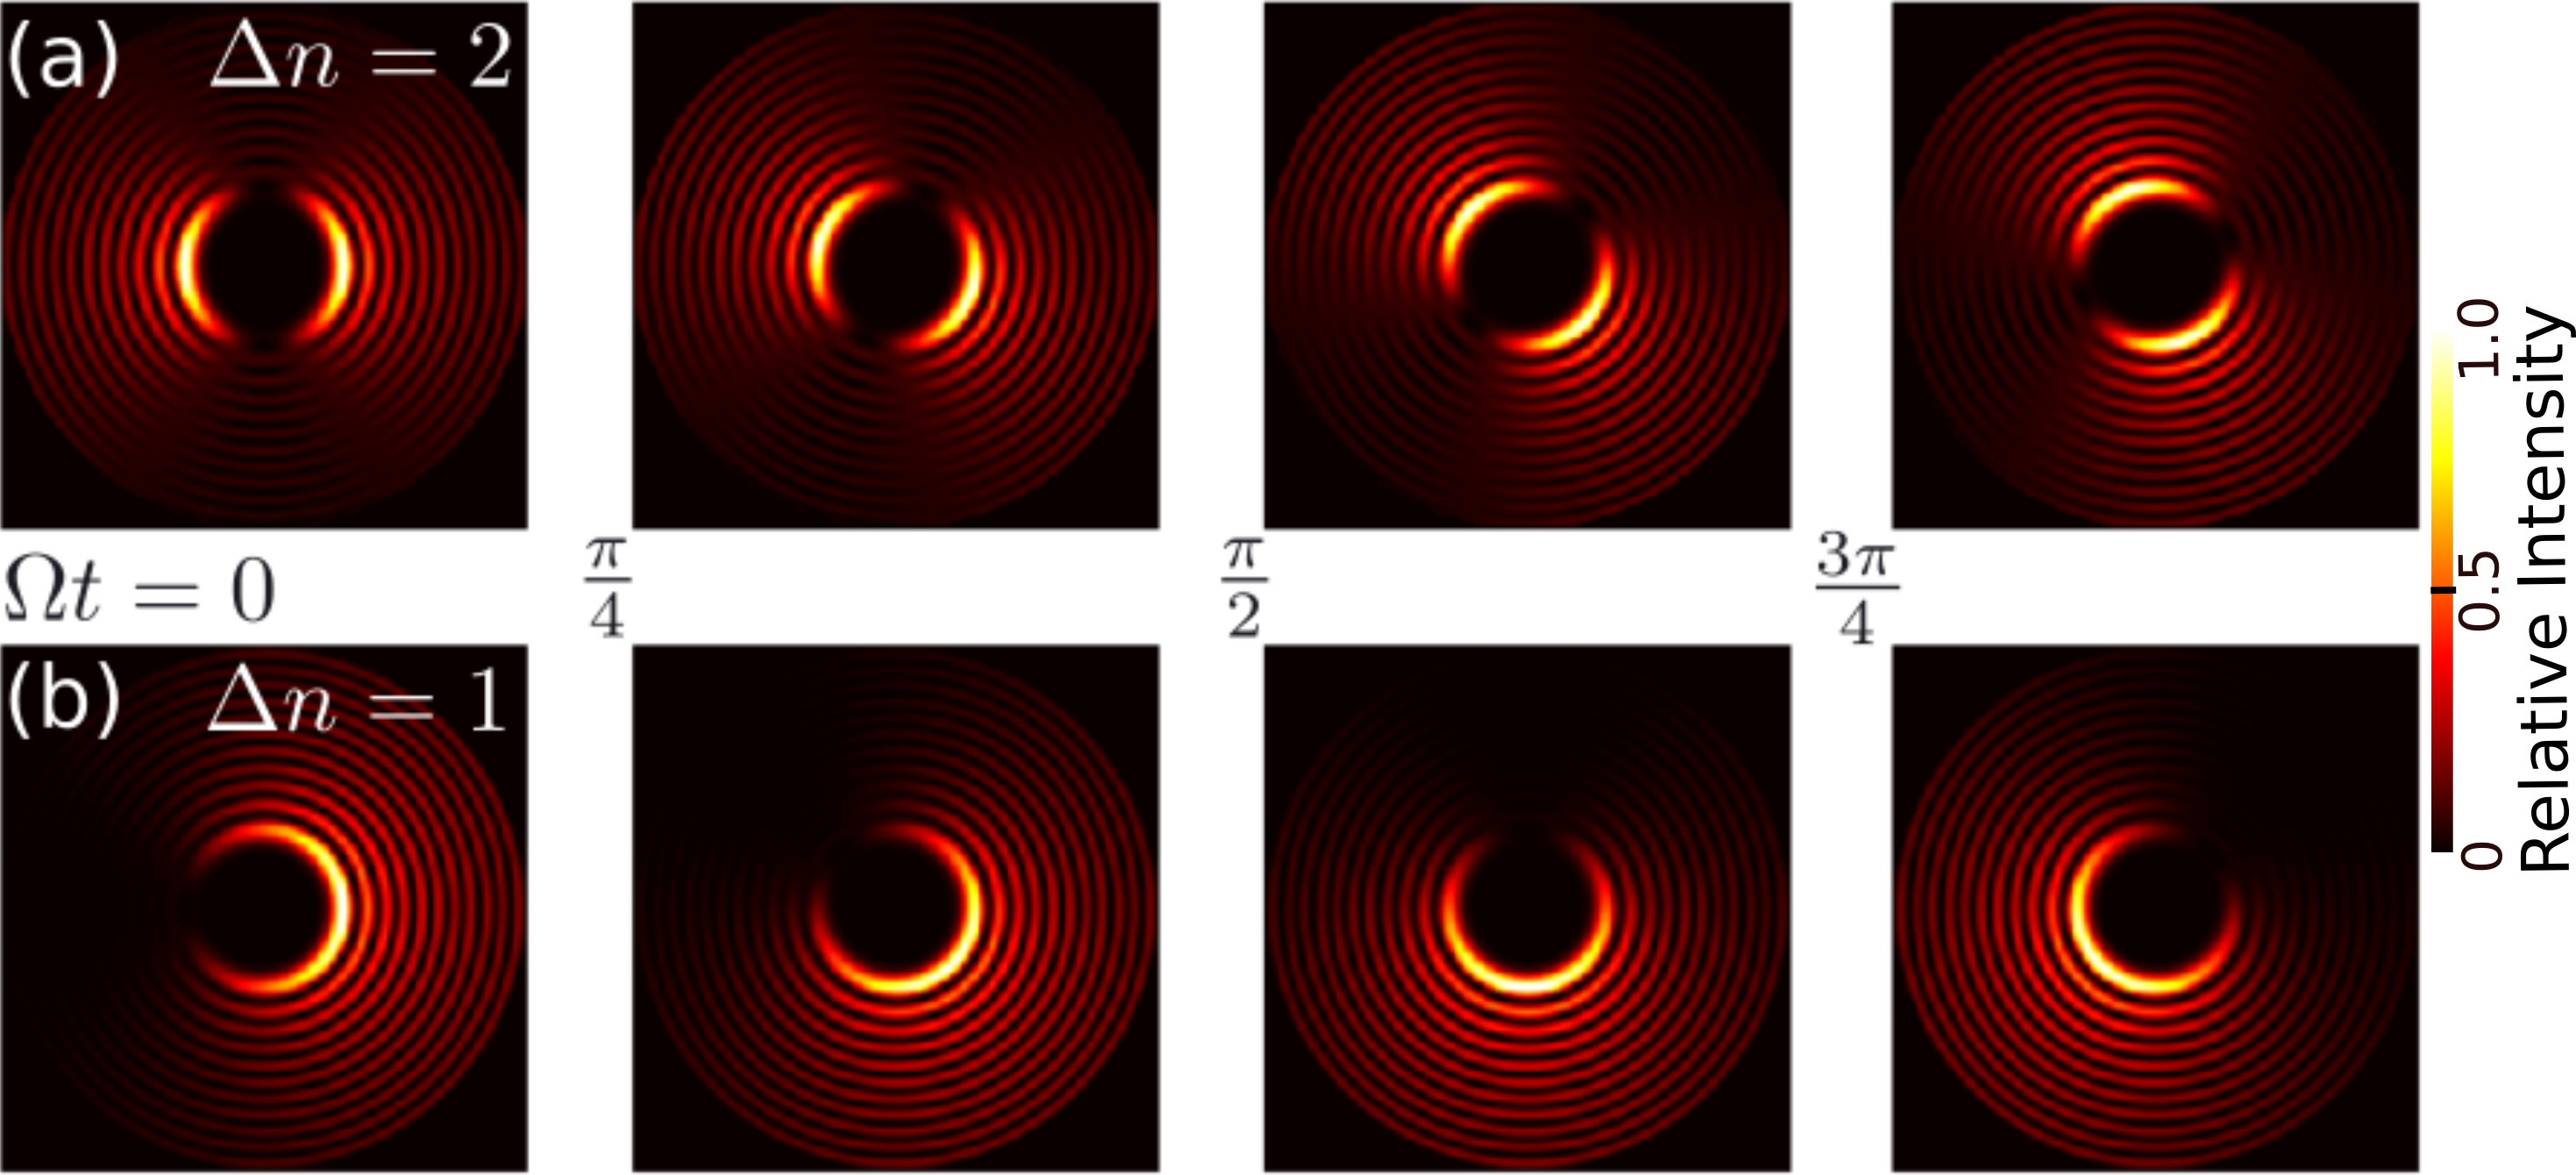
\includegraphics[width=\columnwidth]{rotation03}
  \caption{Rotation of solenoidal states with $n = 6$, $\nu = 15$,
    and $\nu' = \nu - 1$.  (a) Non-accelerating wave packet with
    $\Delta n = n' - n = 2$.
    (b) Accelerating state with $\Delta n = 1$.}
  \label{fig:solenoidalwave}
\end{figure}

Although individual Bessel eigenmodes are time-invariant,
some of their superpositions have probability densities that
rotate at a uniform rate without otherwise
distorting \cite{vasilyeu09,lee10,schulze15}.
Some of these rotating wave packets
constitute accelerating states in the sense that the
expectation value of the particle's position traces out an
accelerating trajectory.
These are not simply related to two-dimensional
Airy states or to related Matthieu and Weber states
\cite{zhang12nonparaxial} or to their generalizations
\cite{bandres13,chremmos13,zhao15shaping}, and thus constitute a distinct class
of accelerating states in two dimensions.

Minimal examples of rotating wave packets
can be constructed by superposing two Bessel states:
\begin{equation}
  \label{eq:solenoid}
  \Psi(\vec{r}, t)
  =
  \frac{1}{\sqrt{2}} \, \left[
    \Psi_{n,\nu}(\vec{r}, t) +
    \Psi_{n', \nu'}(\vec{r}, t)
  \right].
\end{equation}
For clarity, we arrange indices so that $\Delta n = n' - n > 0$.
This superposition's probability density
\begin{multline}
  \rho(\vec{r}, t)
  =
  \frac{1}{2} \, 
  \left[ \rho_{n,\nu}(\vec{r}) + \rho_{n',\nu'}(\vec{r}) \right] + \\
  \left[ \rho_{n,\nu}(\vec{r}) \rho_{n',\nu'}(\vec{r}) \right]^{1/2} \,
    \cos\left( \Delta n[ \phi - \Omega t] \right),
\end{multline}
rotates around the origin with an angular frequency
\begin{equation}
  \label{eq:frequency}
  \Omega = \frac{\hbar}{2m R^2} \,
  \frac{j_{n',\nu'}^2 - j_{n,\nu}^2}{\Delta n}.
\end{equation}
Aside from this rotation, the state neither broadens nor
otherwise distorts.
The resulting periodic recurrence differs from the
breathing modes identified in generalized Airy states
\cite{kaminer12}.
Instead, it closely resembles the discrete
propagation invariance of rotating optical modes \cite{tervo01},
particularly solenoidal beams \cite{lee10}.
For this reason, we refer to the rotating
wave functions described by Eq.~\eqref{eq:solenoid} as
solenoidal states.
Figure~\ref{fig:solenoidalwave} shows the time evolution of
two illustrative examples.

Most solenoidal wave packets are not accelerating states in the sense
identified by Balazs and Berry.
Those with $\Delta n > 1$, such as the example
in Fig.~\ref{fig:solenoidalwave}(a), are symmetric about the origin;
the expectation value of the particle's position coincides with
the center of the box.
Classically, therefore, such states resemble their constituent Bessel states
in that the particle remains motionless at the origin even as its
probability density rotates.

Solenoidal states with $\Delta n = 1$ are asymmetric,
as can be seen in Fig.~\ref{fig:solenoidalwave}(b).
The expectation value for the particle's position,
\begin{equation}
  \label{eq:position}
  \braket{\vec{r}(t)}
  =
  \alpha R \,
  \left[\cos(\Omega t) \, \hat{x} + \sin(\Omega t) \,
    \hat{y}\right], 
\end{equation}
undergoes uniform circulation motion at angular frequency
$\Omega$ and radius $\braket{r} = \alpha R$,
where
\begin{subequations}
  \label{eq:radius}
\begin{align}
  \alpha
  & =
  \frac {
    \int_0^1 J_{n+1}(j_{n+1,\nu'} x) \, J_n(j_{n, \nu} x) \, x^2 \, dx
  }{
    J_{n+2}(j_{n+1,\nu'}) \, J_{n+1}(j_{n,\nu})} \\
  & =
   \frac{2 j_{n+1,\nu'} j_{n,\nu}}{(j_{n+1,\nu'}^2 - j_{n,\nu}^2)^2}.
\end{align}
\end{subequations}
This seems remarkable because
no force acts on the particle within the box.
Such force-free acceleration appears
to violate Ehrenfest's theorem, which relates the expectation value of the
particle's acceleration to the expectation value of the force acting
on the particle,
\begin{equation}
  \label{eq:ehrenfest}
  \frac{d^2 \braket{\vec{r}(t)}}{dt^2}
  = \frac{1}{m} \braket{\vec{F}(\vec{r}(t))}.
\end{equation}
In the present case, $\vec{F}(\braket{\vec{r}(t)}) = 0$ in the force-free
region within the box, but
\begin{equation}
  \label{eq:violation}
  \frac{d^2 \braket{\vec{r}(t)}}{dt^2}
  =
  - \alpha R \, \Omega^2 \hat{r}.
\end{equation}
The apparent discrepancy can be explained because
$\vec{F}(\braket{\vec{r}(t)}) \neq \braket{\vec{F}(\vec{r}(t))}$.

\begin{figure*}[!t]
  \centering
  \includegraphics[width=0.95\textwidth]{light05}
  \caption{Optical realization of accelerating solenoidal states.
    Volumetric reconstructions of asymmetric solenoidal waves
    described by Eq.~\eqref{eq:solenoid} with $\Delta n = 1$.
    (a) Positive helicity: $n = 20$, $\nu = 15$, $\nu' = 14$.
    (b) Negative helicity: $\nu = 14$, $\nu' = 15$.
    (c) Four-mode ($n = 10$, 11, 12, 13) superposition yielding improved in-plane localization.}
  \label{fig:light}
\end{figure*}

The integrability of the solenoidal wave packets comes at
the cost of applying the boundary condition from Eq.~\eqref{eq:boundarycondition}
at $r = R$.
The confined particle exerts a pressure on the wall,
\begin{subequations}
  \label{eq:force}
  \begin{align}
    \label{eq:pressureprinciple}
    P
    & =
      - \frac{1}{2 \pi R} \frac{d E}{d R} \\
    & =
      \frac{\hbar^2}{4 \pi m R^4}
      \left(
      j_{n+1,\nu'}^2 + j_{n,\nu}^2
      \right).
      \label{eq:pressureactual}
  \end{align}
\end{subequations}
By Newton's third law, the wall exerts a complementary
force on the wave packet that is directed radially inward.
When averaged over angles, the net force acting on the
particle located at $\braket{\vec{r}}$ is
\begin{subequations}
  \label{eq:forceactual}
\begin{equation}
  \braket{\vec{F}(\vec{r})}
  = 
  - \beta R \, P \, \hat{r} ,
\end{equation}
where
\begin{align}
  \beta
  & =
    \lim_{\epsilon \to 0}
    \frac{\left.
    \int_0^{2\pi} \rho(\vec{r},t) \cos(\phi - \Omega t) \, d\phi
    \right\vert_{r = R - \epsilon}}
    {\left.
    \int_0^{2\pi} \rho(\vec{r},t) \, d\phi
    \right\vert_{r = R - \epsilon}} \\
  & =
    \frac{2 j_{n+1,\nu'}j_{n,\nu}}{
    j_{n+1,\nu'}^2 + j_{n,\nu}^2} .
\end{align}
\end{subequations}
Comparison with Eq.~\eqref{eq:violation} confirms
that Ehrenfest's theorem is satisfied: the force
responsible for the particle's classical circular
motion is exerted by the wave function's interaction
with the bounding wall.

In principle, accelerating solenoidal states can be prepared
as superpositions of Bessel beams without confining boundary conditions.
Such unconfined states rotate without a central force, and
so appear to violate Ehrenfest's theorem.
Because Bessel states
are not square-integrable, however, they are best
interpreted as superpositions of plane-wave states
\cite{balazs79}.
The rotation of solenoidal wave packets then 
represents the ensemble-averaged behavior of
multiple particles' non-accelerating trajectories.

The possibility of Ehrenfest violations arises again
for normalizable approximations to unconfined
solenoidal wave packets that are prepared by truncating
$\Psi(\vec{r},t)$ at $r = R$.
These truncated wave packets still appear to rotate,
and they evolve under truly force-free conditions.
To illustrate this phenomenon, Fig.~\ref{fig:light}
presents optical analogs of truncated solenoidal states.
We prepare these solenoidal beams of light
by using intermediate-plane holograms \cite{mondal18}
to convert the linearly polarized
Gaussian TEM$_{00}$ beam from
a solid state laser (Coherent Verdi 5W) into a superposition
of helical Bessel modes of the form described by
Eq.~\eqref{eq:solenoid}.
The mode-converting holograms are imprinted
on the beam with a phase-only liquid crystal 
spatial light modulator (Hamamatsu X10468-16).

Figure~\ref{fig:light}(a) and Fig.~\ref{fig:light}(b)
show volumetric reconstructions of two
solenoidal laser beams with $\Delta n = 1$.
The data for these reconstructions
were obtained by translating a video camera 
(NEC TI-324AII) along the optical axis and
combining the resulting stack of images.
Each reconstruction shows three complete cycles of shape-preserving
propagation.
The solenoid in Fig.~\ref{fig:light}(a) has a right-handed twist
while that in Fig.~\ref{fig:light}(b) is left-handed.
Each volumetric reconstruction is paired with three
transverse slices from the planes labeled
(i), (ii) and (iii) in the renderings.
These slices show three stages in the
intensity distributions' rotation about the optical axis at
\SI{120}{\degree} intervals.
Additional planes in the renderings
correspond to each of the three complete rotations
captured over the
course of \SI{1}{\meter} of propagation.  The full non-diffracting
range of these beams extends beyond \SI{2}{\meter}.

The two-state superpositions discussed so far are not
the only accelerating wave packets.
Figure~\ref{fig:light}(c) shows a four-state superposition
designed to optimally localize the wave packet as it spirals
around the origin.
In this case, there can be no doubt that the point of
maximum intensity rotates about the 
optical axis, and therefore that
the most probable particle position,
$\vec{r}^\ast(t)$, undergoes uniform
circular motion under force-free conditions.

Figure~\ref{fig:translation}(a)
shows a representative simulation of
$\vec{r}^\ast(t)$ superimposed on a snapshot
of the initial distribution, $\rho(\vec{r},0)$.
Figure~\ref{fig:translation}(b) shows the corresponding
experimental measurement of $\vec{r}^\ast(z)$.
The angular position of the peak, $\theta^\ast(t)$,
advances uniformly, as can be seen in Fig.~\ref{fig:translation}(c).
For clarity, we have scaled the simulation time to best
superimpose the temporal evolution of the simulation
data on the spatial evolution of the experimental data, $\theta^\ast(z)$.

This apparent contradiction of the Ehrenfest theorem
is resolved by tracking the mean particle position,
$\braket{\vec{r}(t)}$, which also is plotted
in Fig.~\ref{fig:translation}.
Results for $\braket{x(t)}$ and $\braket{x(z)}$ are plotted in
Fig.~\ref{fig:translation}(d), with the simulation
time again scaled as in Fig.~\ref{fig:translation}(c).
In both simulation and experiment, the
classical trajectory of the unconfined
rotating wave packet actually \emph{translates}
steadily away from the beam's axis with an
impact parameter, $b$ set by the average position
at $t = 0$.
This motion arises because the truncated
wave packet diffracts beyond $r = R$ by precisely
the amount needed to conserve momentum
under force-free conditions.
The nature of the state's time 
evolution is masked because diffraction has
little apparent influence on the wave packet's
structure at early times, particularly near
the center of the system.
Remarkably, this means that the 
finite-aperture solenoidal laser modes
presented in Fig.~\ref{fig:light} are not
accelerating states in the sense introduced
by Balasz and Berry, despite their
apparent rotation.

\begin{figure}
  \centering
  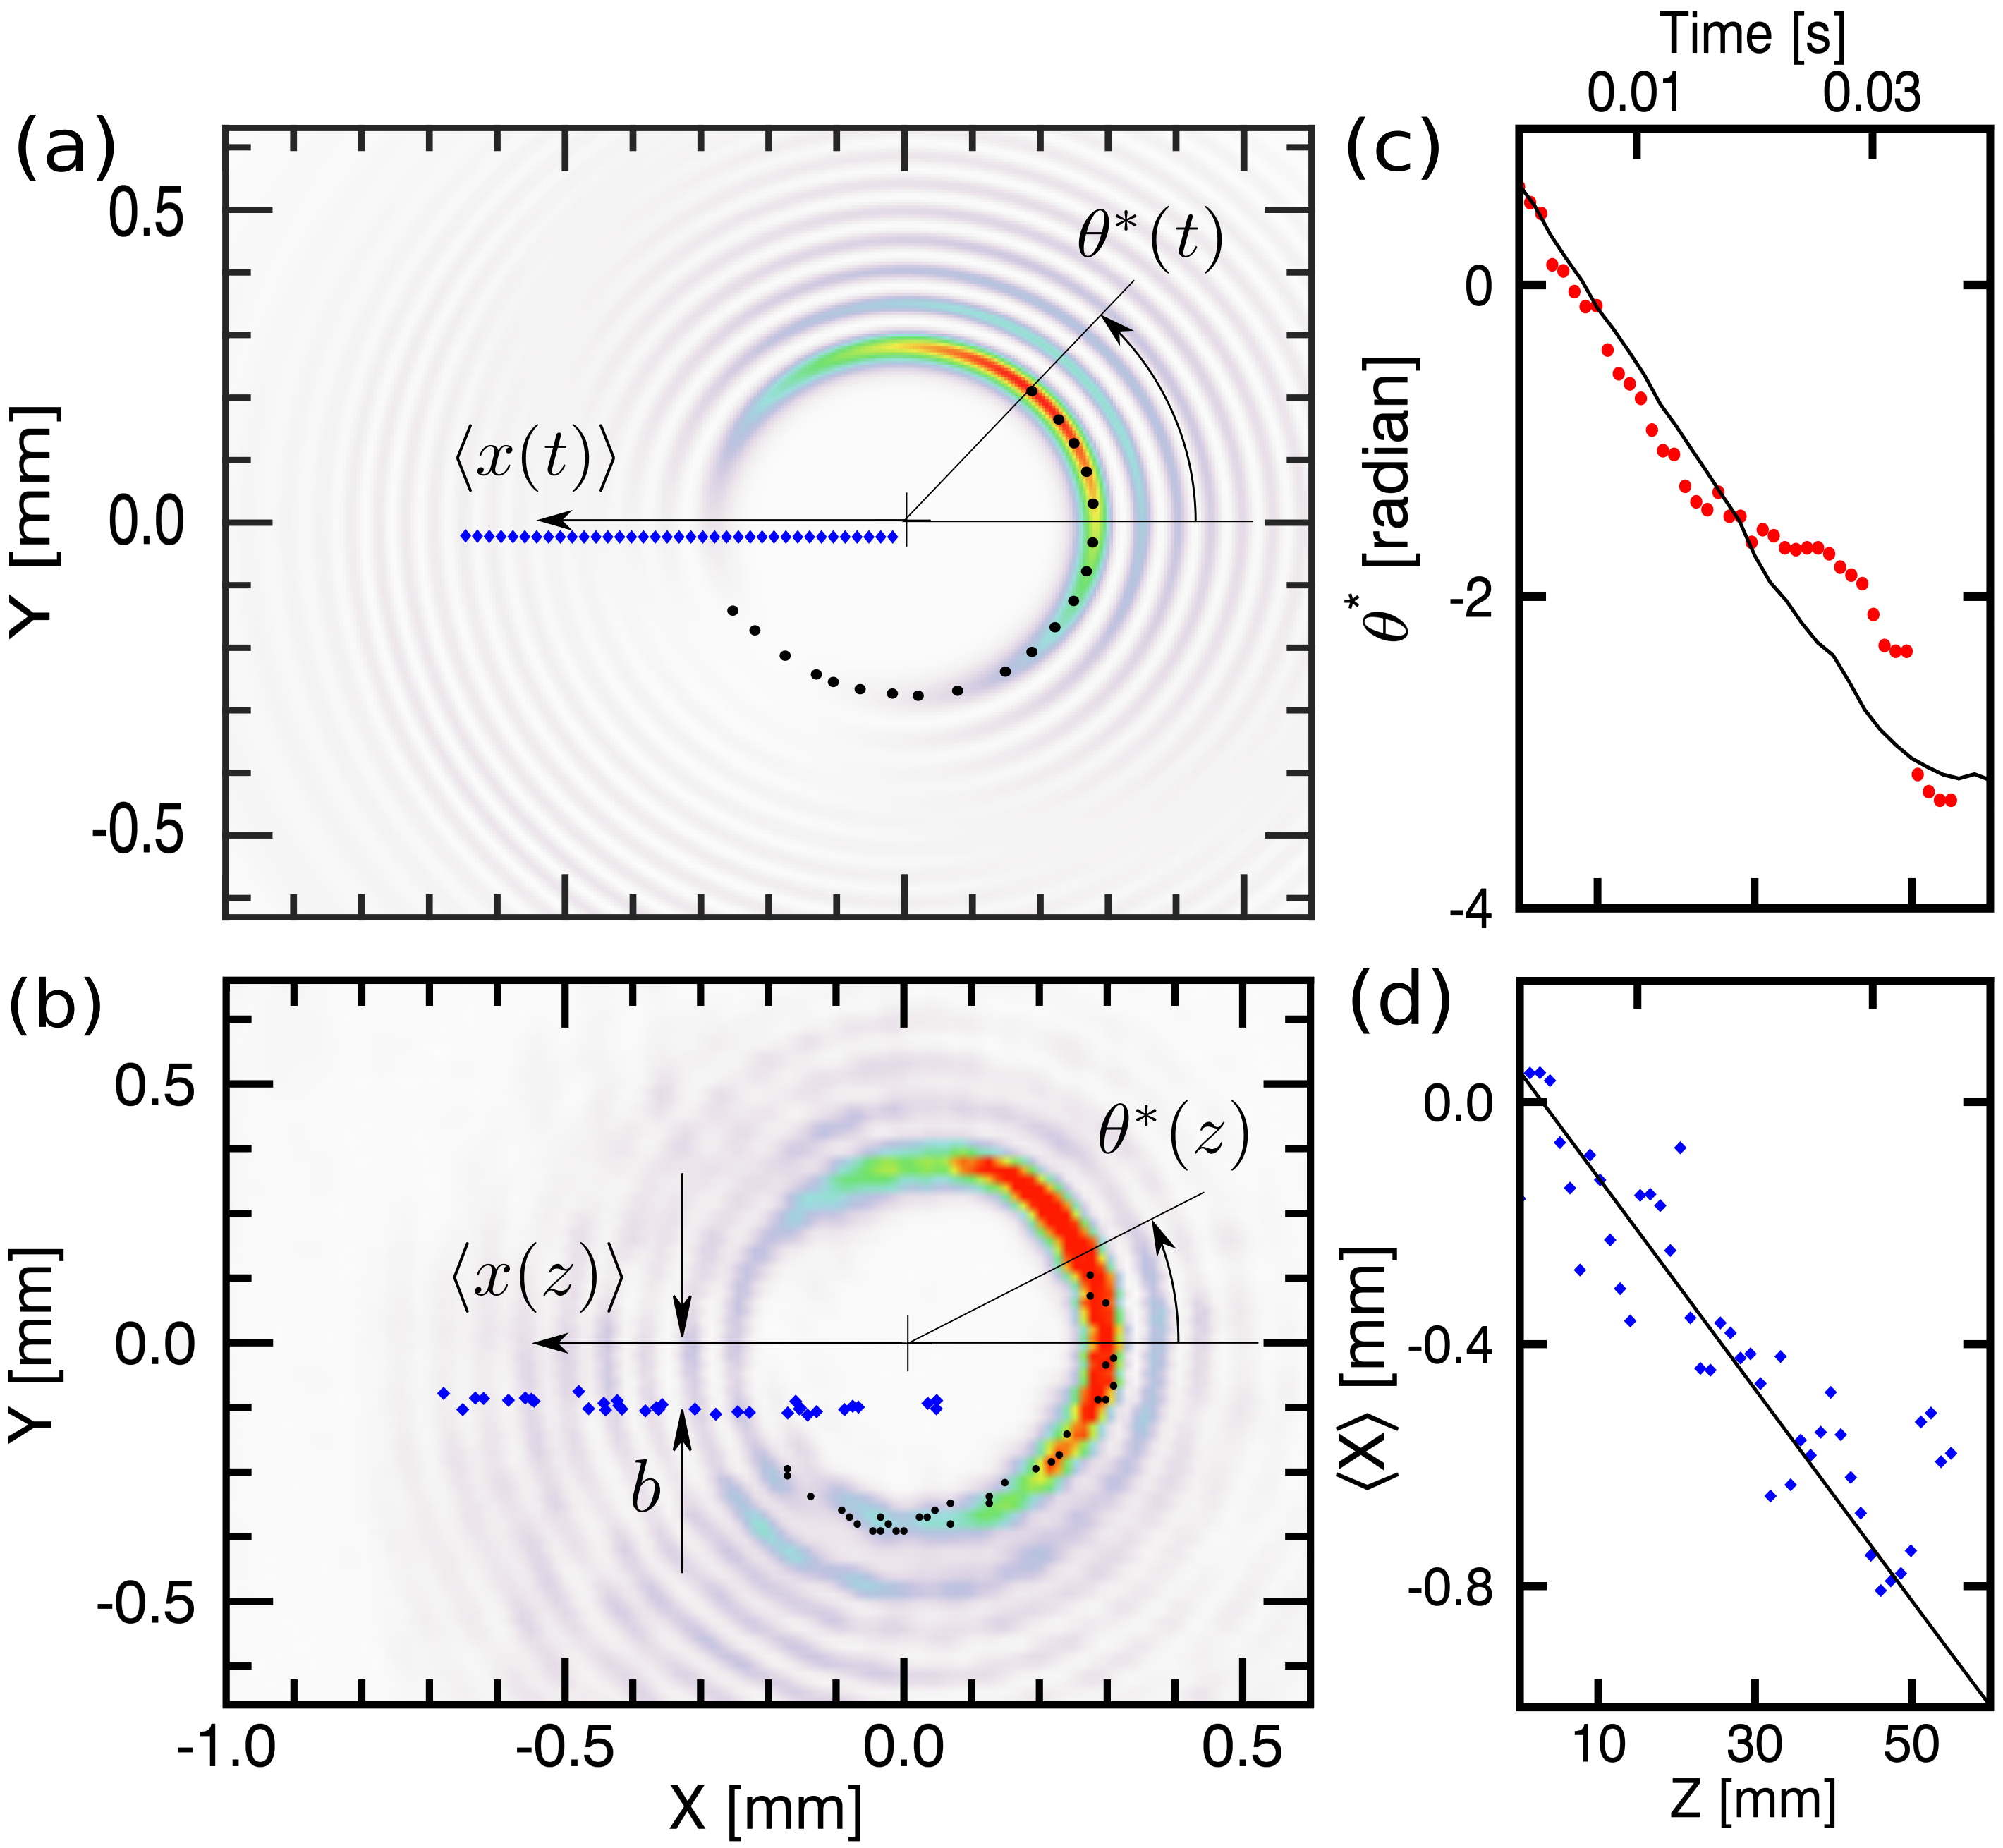
\includegraphics[width=\columnwidth]{translation05}
  \caption{Translation of a rotating wave packet.
  (a) Simulation of an accelerating state with $n = 20$, 
  $\nu = 16$ and $\nu' = 17$.  The image shows a region of interest
  around the center of
  the probability density $\rho(\vec{r},t)$.  Discrete points show
  the time evolution of the the most probable 
  position $\vec{r}^\ast(t)$, which circulates, 
  and of the expectation value
  of the position $\braket{\vec{r}(t)}$, which translates.
  (b) Corresponding experimental realization.
  (c) Time evolution of the mode position $\theta^\ast(t)$
  in the simulation (solid curve) compared with 
  $\theta^\ast(z)$ from the experimental data (discrete points).
  (d) Time evolution of the simulated wave packet's mean position
  $\braket{x(t)}$ compared with the position of the experimental
  center of brightness, $\braket{x(z)}$.
  }
  \label{fig:translation}
\end{figure}

Although the confined particle's classical acceleration
can be accounted for by the influence
of boundary conditions,
its rate of circulation is less straightforward to interpret.
The classical angular momentum carried by an
accelerating solenoidal wave packet is
\begin{subequations}
  \label{eq:Lz}
  \begin{align}
    \label{eq:solenoidLz}
    L_z^{(c)}
    & = m \alpha^2 R^2 \Omega \\
    & =
      2 \frac{j_{n+1,\nu'}^2 j_{n,\nu}^2}{
      (j_{n + 1,\nu'}^2 - j_{n,\nu}^2)^3} \, \hbar ,
  \end{align}
\end{subequations}
which differs from the state's quantum mechanical angular momentum,
\begin{equation}
  \label{eq:solenoidQLz}
  \braket{L_z} = \left(n + \frac{1}{2} \right) \hbar.
\end{equation}
Indeed, $L_z^{(c)}$ and $\braket{L_z}$ can have opposite signs
depending on the choice of radial quantum numbers $\nu$ and $\nu'$.
The solenoidal states represented in Figs.~\ref{fig:light}(a) 
and \ref{fig:light}(b), for example, 
have opposite classical angular
momentum even though they carry the same quantum mechanical
angular momentum.
Unconfined solenoidal states also carry classical angular
momentum
\begin{equation}
L_z^{(c)} 
=
m 
\left[\braket{\vec{r}(0)} \times \frac{d \braket{\vec{r}(t)}}{dt}\right]
\cdot \hat{z}
\end{equation}
that is equal to the confined value from
Eq.~\eqref{eq:Lz}
and generally differs from the quantum-mechanical
value, Eq.~\eqref{eq:solenoidQLz}.
Similar discrepancies between classical and quantum mechanical
angular momenta have been been observed in the spatial structure
of holographically-patterned electron
beams \cite{schattschneider14}.
A comprehensive paradigm for understanding these discrepancies and their physical consequences remains elusive.


\section{Acknowledgment}
This work was supported primarily
by the National Science Foundation under award number
DMR-1305875 and in part by the MRSEC program
of the NSF through award number
DMR-1420073.
The authors are grateful for helpful conversations
with David Pine, Paul Chaikin and
Aaron Yevick.


   \newpage
  
   \chapter{Conclusions}
\label{ch:conclusion}

This thesis has introduced a new technique, 
Intermediate-plane holography that is particularly useful for projecting
modes whose ideal Fresnel holograms are dominated by large
amplitude variations, and so suffer from low diffraction efficiency.
In addition to improving diffraction efficiency, shifting the
hologram plane also can improve mode purity by moving the
length scale for phase variations into the spatial bandwidth of a
practical diffractive optical element.
Both of these considerations figure in the success of intermediate-plane
holograms for projecting Bessel beams and their superpositions.
Because Bessel beams are the natural basis for propagation-invariant
modes, intermediate-plane holography lends itself naturally
to long-range projection.
We have demonstrated meter-scale projection using centimeter-scale
optical elements.
These same elements have additional potential applications for
topologically multiplexing and demultiplexing non-diffracting modes
for optical communications \cite{gibson04,bozinovic13,willner15}.
The same ability to project sophisticated superpositions of
topological modes could have additional applications to remote
sensing and LIDAR \cite{cvijetic15}.
Finally, the same principals discussed here in the context of
optical holography should apply equally well to other types
of waves, most notably to acoustic waves. As for future research,
intermediate plane holography can be utilized to create braided
or knotted optical field.

We believe that the material presented in this thesis will serve as a guide for further advancement in  designing optical modes of light using SLM with better mode purity and diffraction efficiency. It will also be a stepping stone to understand and realize kilometer scale tractor beam.
   \newpage

    %%%%% Appendices start %%%%%%%%%%%%%%%%
    %% Comment out the following line if your thesis has no appendix
    % \appendix
    
    %If you have only one appendix copy this line out
    %% \phantomsection
    %% \addcontentsline{toc}{chapter}{Appendices}
    
    % 
    % If you have multiple appendices, they shouldn't individually appear
    % in the table of contents, but rather be listed in the List of
    % appendices. To do this, put the following code(defined in
    % definitions.tex) at the front of each appendix file(Tip from Jan Smrek):
    %
    % %\SkipTocEntry\chapter{Appendix Title} 
    % %\label{app:appendixtitle}
    % %\appcaption{\thechapter \space Appendix Title}
    %
    %\include{appendix}
%
%    \begin{appendices}      
%      \include{Chapters/appendix_01_camera}
%      %\include{Chapters/appendix_02_lorenzmie_approx}
%      \include{Chapters/appendix_02_discretize_dw}
%     \end{appendices}

    

    \clearpage

%\addcontentsline{toc}{chapter}{Reference}
%\singlespacing
\renewcommand{\bibname}{Bibliography}
\nocite{apsrev41Control}
\bibliographystyle{apsrev4-1}
\bibliography{Bibliography/abbreviations,Bibliography/argha,Bibliography/dgg,Bibliography/grier,Bibliography/tweezer,Bibliography/accelerating}

\end{document}
